\documentclass[11pt,letterpaper]{article}
\usepackage{graphicx, geometry, amsmath, hyperref, url, natbib, booktabs, xcolor, listings}
\usepackage{longtable}
\usepackage{array}
\usepackage{makecell}
\geometry{margin=1in}
\hypersetup{colorlinks=true, linkcolor=black, citecolor=black, urlcolor=black}

\newcommand{\cscore}{\texttt{c\_score}}
\newcommand{\cscorealign}{\texttt{c\_score\_align}}

\title{Gold-Free Faithfulness Metrics for NL-to-FOL Translation\\[0.5em]\large Internal Research Report}
\author{AI Inventor Research}
\date{September 2026}

\begin{document}
\maketitle
\tableofcontents
\newpage

%% ====================================================================
\section{Framing}
%% ====================================================================

Translating natural language into first-order logic (NL-FOL) is a prerequisite for neurosymbolic reasoning pipelines~[10], yet evaluating whether a candidate formula faithfully captures a sentence's meaning remains an open problem. Gold FOL annotations are expensive, non-unique, and unreliable: Brunello et al.~[3] found that approximately 42\% of entries in both FOLIO~[1] and MALLS~[2] contain incorrect formalisations. Existing metrics either require a gold formula (exact match, prover-checked equivalence) or only verify that the output parses~[5,~6]. The user's own pilot study used structural consistency checks (arity agreement, predicate-set overlap across reruns, joint satisfiability) that measure stability but not whether a formula says what its sentence says.

This run investigates gold-free metrics that predict faithfulness to the text given only a sentence and a candidate formula, with no reference formula, no ontology, and no domain knowledge. The evaluation is a meta-evaluation: we build a labelled set of (sentence, formula) pairs from public benchmarks whose gold has been audited, and measure each metric's ability to discriminate correct translations from errors.

%% ====================================================================
\section{Iteration 1}
%% ====================================================================

\subsection{Strategy}

The iteration screens four candidate metric families head-to-head on a frozen evaluation set, with a disguised cheap LLM judge as the bar to beat.

\textbf{Candidates.} (A) FOL-Triage, a three-layer cascade: L1 (formula lint: deterministic formula smells), L2 (text accounting: bag-of-words and role-aware coverage), and L3 (role questionnaire: a small LLM reads the text and z3 reads the formula; their structured answers are compared). (B) Round-trip verification: verbalise the formula back to natural language and compare to the original via NLI or embedding similarity~[7]. (C) Cross-system consensus: collect translations of the same sentence from multiple independent systems, measure z3-equivalence between the candidate and the peer pool, and score disagreement~[8]. (D) Disguised cheap judge and baselines: an LLM judge, structural pilot metrics, and round-trip features evaluated on nonce-disguised sentences to control for memorisation.

\textbf{Evaluation set.} The frozen screen uses Logic-LM~[10] released outputs on FOLIO validation: three LLM systems (GPT-3.5-turbo, GPT-4, text-davinci-003) producing 796 items. Track L contains LLM outputs labelled by z3 equivalence to corrected gold~[4]; track H contains the 294 original human gold formulas, of which 57 are errors according to the corrected labels. The parallel run measured 43.9\% of solver-non-equivalent candidates as faithful by a three-family panel; iteration~2 re-scores with those adjudicated labels.

\textbf{Decision rule.} A candidate must achieve AUROC $\geq 0.65$ on track L (ERROR vs CORRECT), with coverage $\geq 90\%$, rewrite false-alarm rate $\leq 10\%$ per rewrite family, and cost $\leq \$0.002$ per item. It advances only if its AUROC exceeds the disguised cheap judge's, with a paired bootstrap CI excluding zero.

\textbf{Development dataset (Artifact E).} A separate 700-sentence, 8,507-row development set was constructed from FOLIO training premises, MALLS training long/conditional/exception strata, and FOLIO curated conclusions, each translated by 9 LLM families plus ccg2lambda plus GPT-4 gold. Labels were assigned by z3 equivalence to audited gold, with contested cases adjudicated by a three-member panel (Claude Haiku-4.5, GLM-4.6, Kimi-K2). This set is reserved for iteration~2 confirmation.% gen_art_dataset_1
\footnote{Artifact \texttt{gen\_art\_dataset\_1}. Code: \url{https://github.com/ai-inventor-papers/ai-invention-eff060-layered-gold-free-checks-for-logic/tree/fork/run_qck1d05BqxkX/round-1/dataset-1}}

The dataset contains 1,750 CORRECT, 5,005 ERROR, 1,086 UNPARSEABLE, 276 UNRESOLVED, and 390 CONTESTED items. The panel calibration subset (173 items) shows that the panel agrees with expert-corrected labels on both faithful and unfaithful items. A screen audit of 1,173 items from the Logic-LM screen confirms the label assignment. The dataset cost \$9.83 in API calls.

%% ------------------------------------------------------------------
\subsection{Experiment A: FOL-Triage}
%% ------------------------------------------------------------------

FOL-Triage was evaluated on the frozen screen with Gemini 2.5 Flash Lite as the primary LLM for L3. Total API spend was \$0.29.% gen_art_experiment_1
\footnote{Artifact \texttt{gen\_art\_experiment\_1}. Code: \url{https://github.com/ai-inventor-papers/ai-invention-eff060-layered-gold-free-checks-for-logic/tree/fork/run_qck1d05BqxkX/round-1/experiment-1}}

\subsubsection{Headline AUROCs (track L, ERROR vs CORRECT, $n=477$, 199 errors)}

\begin{table}[!htbp]
\centering
\caption{FOL-Triage headline AUROCs on track~L (Iteration~1, Experiment~A).}
\label{tab:foltriage_headline}
\begin{tabular}{lrrr}
\toprule
Metric & AUROC & 95\% CI & AUPRC \\
\midrule
L1 (any smell) & 0.508 & [0.499, 0.519] & 0.425 \\
L2 bag-of-words & 0.737 & [0.677, 0.801] & 0.690 \\
L2 role-aware & 0.557 & [0.527, 0.594] & 0.476 \\
L3 score & 0.756 & [0.701, 0.809] & 0.657 \\
Fused (fitted on H, no leak) & 0.759 & [0.695, 0.825] & 0.740 \\
Fused (all H) & 0.827 & [0.778, 0.874] & 0.771 \\
Fused (cross-fit L) & 0.864 & [0.824, 0.902] & 0.789 \\
Decomposed judge (LLM reads formula) & 0.716 & [0.645, 0.789] & 0.717 \\
L3 with local Qwen2.5-1.5B & 0.708 & [0.637, 0.774] & 0.603 \\
\bottomrule
\end{tabular}
\end{table}

The primary no-leak fused score is 0.759. The fused-all-H and cross-fit-L numbers (0.827, 0.864) are shown for completeness but are not valid held-out estimates: the former uses the full track H for fitting, and the latter is a within-L cross-fit that overstates generalisation.

\textbf{Track H (human gold errors, $n=258$, 57 errors).} Fused out-of-fold AUROC is 0.777 [0.698, 0.847]. L1 alone reaches 0.655, compared to 0.508 on track L. The lint rules fire on human annotation errors but not on LLM outputs, because the two populations produce different formula smells.

\subsubsection{L1 lint: a negative result on LLM outputs}

L1 flags formulas with deterministic smells (existential implication, free variables, arity clashes, vacuity, trivial formulas, dangling predicates). On track L, the true positive rate is 2.0\% at a false positive rate of 0.4\%, giving AUROC 0.508. This is a negative result: L1 lint does not transfer from human annotation errors (where it is effective, AUROC 0.655) to LLM outputs. The reason is that LLM-generated formulas rarely contain the syntactic pathologies L1 detects; their errors are semantic (wrong predicates, missing conditions, scope mistakes).

All nine individual smell rules have false-alarm rates below 3\% on every system:

\begin{table}[!htbp]
\centering
\caption{L1 lint per-smell false-alarm rates by system (Iteration~1, Experiment~A).}
\label{tab:l1_smell_fa}
\begin{tabular}{lrrr}
\toprule
Smell & gpt-3.5 FA & gpt-4 FA & davinci-003 FA \\
\midrule
EX\_IMP & 0.0 & 0.0 & 0.0 \\
ALL\_AND & 0.0 & 0.0 & 0.0 \\
IFF\_RESTR & 0.0 & 0.009 & 0.0 \\
GLUE & 0.0 & 0.0 & 0.0 \\
FREE & 0.0 & 0.0 & 0.0 \\
VACUOUS & 0.0 & 0.0 & 0.0 \\
TRIVIAL & 0.0 & 0.0 & 0.0 \\
ARITY & 0.0 & 0.0 & 0.0 \\
DANGLING & 0.0 & 0.0 & 0.0 \\
\bottomrule
\end{tabular}
\end{table}

Only the FREE smell fires on any track-L errors (4 items).

\subsubsection{L2 role-aware check: below bag-of-words}

The role-aware UD-based check (L2-role) achieves AUROC 0.557, which is 0.18 below the simpler bag-of-words check (L2-bow, 0.737). The role-aware layer adds no discriminative power over word overlap.

\subsubsection{Decomposed judge ablation}

Replacing z3 with an LLM that reads the formula directly (the decomposed judge) drops L3 AUROC from 0.756 to 0.697 ($\Delta$AUROC $= -0.059$). The LLM gets only 57.6\% of binary argument slots correct on track L and 36.4\% on track H. The z3 answerer is significantly more accurate for structured formula reading.

\subsubsection{Per-type sensitivity (track L, at binary threshold)}

\begin{table}[!htbp]
\centering
\caption{FOL-Triage per-type sensitivity on track~L (Iteration~1, Experiment~A).}
\label{tab:pertype_trackL}
{\small
\begin{tabular}{lrrrrrrr}
\toprule
Error type & $n$ & L1 & L2-bow & L2-role & L3 & Fused & Cascade \\
\midrule
NEG & 5 & 0.0 & 0.2 & 1.0 & 0.2 & 0.4 & 1.0 \\
QUANT & 2 & 0.0 & 0.0 & 0.5 & 0.0 & 0.5 & 0.5 \\
CONN & 4 & 0.0 & 0.0 & 0.0 & 0.0 & 0.0 & 0.0 \\
DROP & 142 & 0.028 & 0.479 & 0.127 & 0.197 & 0.599 & 0.606 \\
ADD & 150 & 0.020 & 0.473 & 0.107 & 0.173 & 0.653 & 0.573 \\
SWAP & 12 & 0.0 & 0.0 & 0.083 & 0.25 & 0.083 & 0.333 \\
BIND & 8 & 0.125 & 0.0 & 0.125 & 0.0 & 0.375 & 0.25 \\
COMPOUND & 187 & 0.118 & 0.428 & 0.166 & 0.160 & 0.599 & 0.578 \\
\bottomrule
\end{tabular}
}
\end{table}

FOL-Triage is most sensitive to ADD and DROP errors (the largest categories), with the fused score catching about 60\%. It misses CONN errors entirely (0/4) and detects SWAP poorly (1/12). Negation errors are fully caught by the cascade (which fires L2-role, where monotonicity shifts are visible) but L1 and L2-bow miss them.

\subsubsection{Per-type sensitivity (track H)}

\begin{table}[!htbp]
\centering
\caption{FOL-Triage per-type sensitivity on track~H (Iteration~1, Experiment~A).}
\label{tab:pertype_trackH}
{\small
\begin{tabular}{lrrrrrrr}
\toprule
Error type & $n$ & L1 & L2-bow & L2-role & L3 & Fused & Cascade \\
\midrule
NEG & 4 & 0.0 & 0.0 & 0.25 & 0.0 & 0.25 & 0.25 \\
REV & 1 & 0.0 & 0.0 & 0.0 & 0.0 & 0.0 & 0.0 \\
QUANT & 1 & 0.0 & 0.0 & 0.0 & 0.0 & 0.0 & 0.0 \\
RESTR & 1 & 1.0 & 1.0 & 0.0 & 0.0 & 1.0 & 1.0 \\
CONN & 8 & 0.25 & 0.125 & 0.0 & 0.375 & 0.375 & 0.375 \\
MOVE & 2 & 0.5 & 0.0 & 0.5 & 0.0 & 0.5 & 1.0 \\
DROP & 14 & 0.143 & 0.357 & 0.0 & 0.143 & 0.357 & 0.5 \\
ADD & 19 & 0.158 & 0.368 & 0.053 & 0.211 & 0.526 & 0.579 \\
SWAP & 2 & 0.0 & 0.5 & 0.0 & 0.5 & 0.5 & 0.5 \\
BIND & 1 & 1.0 & 1.0 & 0.0 & 0.0 & 1.0 & 1.0 \\
UNGLUE & 5 & 1.0 & 0.4 & 0.0 & 0.2 & 1.0 & 1.0 \\
COMPOUND & 33 & 0.303 & 0.182 & 0.242 & 0.182 & 0.545 & 0.636 \\
\bottomrule
\end{tabular}
}
\end{table}

On track~H (57 errors), the per-type pattern differs. UNGLUE errors ($n=5$) are caught at 100\% by L1 and the fused score, because they produce detectable formula smells.

\subsubsection{Invariance under meaning-preserving rewrites}

Five rewrite families were tested on 150 track-L CORRECT items.

\begin{table}[!htbp]
\centering
\caption{Rewrite false-alarm and flip rates for FOL-Triage layers (Iteration~1, Experiment~A).}
\label{tab:rewrite_fa}
{\scriptsize
\begin{tabular}{lr*{10}{r}}
\toprule
Rewrite & $n$ & L1 FA & L1 flip & bow FA & bow flip & role FA & role flip & L3 FA & L3 flip & Fused FA & Fused flip \\
\midrule
RENAME & 150 & 0.0 & 0.0 & 0.18 & 0.093 & 0.013 & 0.0 & 0.033 & 0.007 & 0.22 & 0.013 \\
REORDER & 34 & 0.0 & 0.0 & 0.029 & 0.0 & 0.059 & 0.0 & 0.059 & 0.0 & 0.235 & 0.0 \\
DEMORGAN & 33 & 0.0 & 0.0 & 0.030 & 0.0 & 0.061 & 0.0 & 0.030 & 0.030 & 0.182 & 0.061 \\
CONTRA & 40 & 0.025 & 0.025 & 0.10 & 0.0 & 0.025 & 0.025 & 0.025 & 0.0 & 0.275 & 0.0 \\
PRENEX & 1 & 0.0 & 0.0 & 0.0 & 0.0 & 0.0 & 0.0 & 0.0 & 0.0 & 0.0 & 0.0 \\
\bottomrule
\end{tabular}
}
\end{table}

\begin{figure}[!htbp]
  \centering
  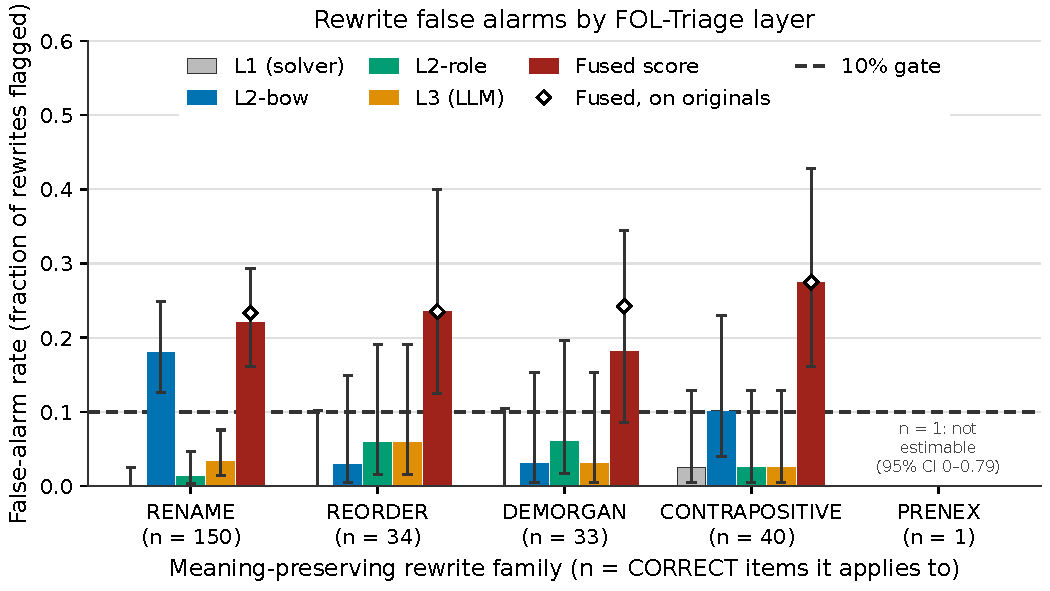
\includegraphics[width=\linewidth,height=0.85\textheight,keepaspectratio]{figures/fig_rewrite_fa_v0.pdf}
  \caption{False-alarm (FA) rate of each FOL-Triage layer under five families of meaning-preserving rewrites, measured on the 150 track-L CORRECT items. Bars give the share of rewritten formulas flagged by L1 lint (grey), L2 bag-of-words (blue), L2 role-aware (green), L3 role schema (amber) and the fused score fitted on track~H (violet); whiskers are Wilson 95\% intervals, and black ticks mark the same layer's FA on the un-rewritten originals. The dashed line is the pre-registered 10\% gate. The fused score fails the gate in every family with $n \geq 33$ (0.18--0.28), but it flags the un-rewritten originals at about the same rate, and its flip rate is at most 0.061.}
  \label{fig:rewrite_fa}
\end{figure}

The rewrite false-alarm gate ($\leq 10\%$ per family) fails. The worst-family fused FA is 0.275 (CONTRAPOSITIVE), but this equals the FA on the original formulas; the flip rate is at most 0.061. The high FA is not caused by the rewrites but by the fused score's calibration: it was fitted on track H where the CORRECT base rate is higher, producing a systematic over-flagging on track L (FA on track-L CORRECT items is 0.194 versus the 0.10 calibration target).

L1, L2-role, and L3 individually pass the 10\% gate. L2-bow fails only under RENAME (FA $= 0.18$), because renaming predicates breaks the bag-of-words match between text and formula.

\subsubsection{Coverage}

\begin{table}[!htbp]
\centering
\caption{FOL-Triage coverage rates (Iteration~1, Experiment~A).}
\label{tab:coverage}
\begin{tabular}{lrrr}
\toprule
Track & $n$ & Parseable & Full coverage rate \\
\midrule
L & 753 & 693 & 0.920 \\
H & 302 & 279 & 0.924 \\
\bottomrule
\end{tabular}
\end{table}

Parse rates by system: gpt-3.5-turbo 0.889, gpt-4 0.946, text-davinci-003 0.921. The coverage gate ($\geq 90\%$) passes.

\subsubsection{Cost}

L1 and L2 are free (CPU-only). L3 costs \$0.175 per 1,000 calls with Gemini 2.5 Flash Lite. The total per-item cost is \$0.0002, passing the \$0.002 gate.

\subsubsection{Contamination check}

L3 was run on nonce-disguised sentences on the full track L. AUROC with exact text-formula alignment: 0.765; with disguised text: 0.770. Paired difference: $-0.005$ [$-0.063$, 0.049]. There is no evidence that the LLM benefits from having seen the public benchmark sentences.

\subsubsection{Complexity strata (track L, fused score)}

\begin{table}[!htbp]
\centering
\caption{Complexity strata AUROCs on track~L (Iteration~1, Experiment~A).}
\label{tab:complexity_strata}
{\small
\begin{tabular}{lrrrr}
\toprule
Stratum & $n$ (error/correct) & Fused AUROC & L2-bow & L3 \\
\midrule
words $< 12$ & 443 (179/264) & 0.781 & 0.742 & 0.772 \\
words 12--19 & 31 (18/13) & 0.521 & 0.596 & 0.541 \\
words $\geq 20$ & 3 (2/1) & 0.500 & 1.000 & 0.000 \\
0 quantifiers & 302 (130/172) & 0.743 & 0.728 & 0.771 \\
1 quantifier & 164 (65/99) & 0.794 & 0.748 & 0.721 \\
$\geq 2$ quantifiers & 11 (4/7) & 0.750 & 0.768 & 0.607 \\
depth $\leq 1$ & 296 (124/172) & 0.762 & 0.745 & 0.779 \\
depth 2--3 & 173 (73/100) & 0.756 & 0.717 & 0.710 \\
depth $\geq 4$ & 8 (2/6) & 0.667 & 0.750 & 0.500 \\
0 conditions & 344 (145/199) & 0.775 & 0.759 & 0.791 \\
1--2 conditions & 131 (54/77) & 0.716 & 0.677 & 0.628 \\
\bottomrule
\end{tabular}
}
\end{table}

The frozen screen is dominated by short, simple sentences (93\% under 12 words). The long and complex strata have too few items to test. This limitation motivates the development dataset (Artifact~E), which oversamples these strata.

\subsubsection{Per-system AUROC (descriptive)}

\begin{table}[!htbp]
\centering
\caption{Per-system AUROCs on track~L (Iteration~1, Experiment~A).}
\label{tab:persystem_auroc}
\begin{tabular}{lrrrrrr}
\toprule
System & $n$ & Error rate & Fused & L1 & L2-bow & L3 \\
\midrule
gpt-3.5-turbo & 143 & 0.378 & 0.689 & 0.500 & 0.650 & 0.722 \\
gpt-4 & 177 & 0.367 & 0.700 & 0.496 & 0.716 & 0.720 \\
text-davinci-003 & 157 & 0.510 & 0.857 & 0.525 & 0.811 & 0.817 \\
\bottomrule
\end{tabular}
\end{table}

FOL-Triage is most discriminative on text-davinci-003, the weakest system.

%% ------------------------------------------------------------------
\subsection{Experiment C: Cross-System Consensus}
%% ------------------------------------------------------------------

The consensus metric collects translations of the same sentence from multiple independent LLM families, checks pairwise z3 equivalence, and scores each candidate by its disagreement with the pool. Total API spend was \$1.52.% gen_art_experiment_3
\footnote{Artifact \texttt{gen\_art\_experiment\_3}. Code: \url{https://github.com/ai-inventor-papers/ai-invention-eff060-layered-gold-free-checks-for-logic/tree/fork/run_qck1d05BqxkX/round-1/experiment-3}}

\subsubsection{Headline AUROCs (track L, ERROR vs CORRECT, $n=546$, 249 errors)}

\begin{table}[!htbp]
\centering
\caption{Consensus metric AUROCs on track~L (Iteration~1, Experiment~C).}
\label{tab:consensus_headline}
{\small
\begin{tabular}{lrrr}
\toprule
Metric & AUROC & 95\% CI & AUPRC \\
\midrule
c\_score (1 $-$ eq\_frac, all peers) & 0.866 & [0.821, 0.906] & 0.827 \\
c\_score (6 fresh peers only) & 0.872 & [0.830, 0.911] & 0.825 \\
c\_score (non-OpenAI peers) & 0.863 & [0.820, 0.903] & 0.808 \\
c\_score (2 Logic-LM peers only) & 0.753 & [0.701, 0.806] & 0.659 \\
medoid depth & 0.722 & [0.673, 0.774] & 0.622 \\
cluster entropy & 0.773 & [0.724, 0.820] & 0.691 \\
SC-5 cheap (gpt-4.1-nano) & 0.725 & [0.669, 0.781] & 0.627 \\
SC-5 same model & 0.716 & [0.632, 0.796] & 0.628 \\
SC-5 entropy & 0.631 & [0.568, 0.693] & 0.539 \\
Pred-set instability (SC) & 0.688 & [0.626, 0.750] & 0.602 \\
Pred-set instability (pool) & 0.770 & [0.717, 0.821] & 0.721 \\
FOL length & 0.527 & [0.470, 0.586] & 0.485 \\
Misalignment (vocab) & 0.835 & [0.794, 0.876] & 0.821 \\
\bottomrule
\end{tabular}
}
\end{table}

\begin{figure}[!htbp]
  \centering
  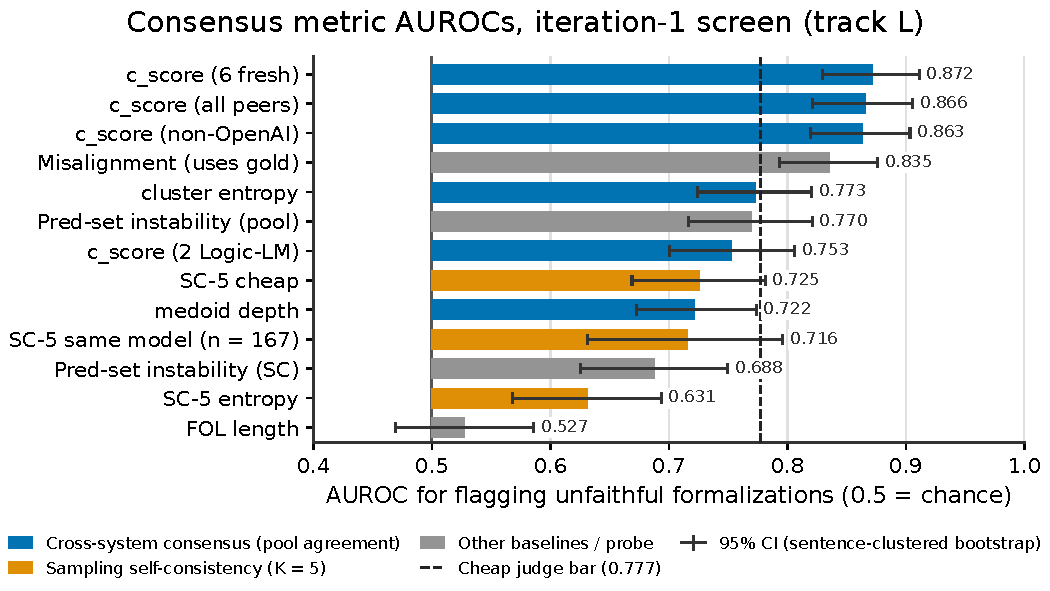
\includegraphics[width=\linewidth,height=0.85\textheight,keepaspectratio]{figures/fig_consensus_auroc_v0.pdf}
  \caption{AUROC (ERROR vs.\ CORRECT) of consensus-based scores and baselines on the iteration-1 frozen screen (track~L, $n=546$, 249 errors). Bars are sorted by AUROC. Dark blue: \texttt{c\_score} variants. Light blue: other pool scores. Orange: self-consistency scores. Grey: FOL length and misalignment probe. The dashed line marks the disguised cheap LLM judge (AUROC 0.777).}
  \label{fig:consensus_auroc}
\end{figure}

The \cscore{} achieves the highest AUROC in the iteration at 0.866. It beats SC-5 (the self-consistency baseline) by $\Delta$AUROC $= +0.140$ [0.085, 0.197]. Using only the six fresh peer translations gives 0.872, slightly higher than using all peers. Restricting to the two other Logic-LM systems drops the AUROC to 0.753, showing that diversity across model families is essential.

\subsubsection{RENAME rewrite invariance: failure}

Under predicate renaming (replacing predicate names with WordNet synonyms or nonce names), the \cscore{} false-alarm rate is 96\% (100\% for constant-only renaming). This is expected and fundamental: two formulas with different predicate names are not z3-equivalent, so any rename breaks the equivalence check.

\subsubsection{Blind-spot analysis}

38\% of ERROR items are z3-equivalent to the medoid (the most popular peer formula). This places a ceiling on recall of approximately 62\%. The blind-spot rate is 5\% for polarity errors and 57\% for structural errors.

\subsubsection{Cost}

The peer pool costs \$0.0015 per sentence (6 peers via API). Total experiment spend: \$1.52. z3 pairwise equivalence checking is free.

%% ------------------------------------------------------------------
\subsection{Experiment D: Disguised Judge and Baselines}
%% ------------------------------------------------------------------

This experiment establishes the bar: every baseline metric and every judge variant on the same shared screen, scored with nonce-disguised sentences to control for memorisation. Total API spend was \$2.02.% gen_art_experiment_4
\footnote{Artifact \texttt{gen\_art\_experiment\_4}. Code: \url{https://github.com/ai-inventor-papers/ai-invention-eff060-layered-gold-free-checks-for-logic/tree/fork/run_qck1d05BqxkX/round-1/experiment-4}}

The primary cheap judge (Gemini 2.5 Flash Lite, JSON 0--100 scoring, nonce-disguised sentences) achieves AUROC 0.777 [0.720, 0.827] on track L ($n=524$, 230 errors, 294 correct).

\begin{table}[!htbp]
\centering
\caption{Full baseline table on track~L (Iteration~1, Experiment~D).}
\label{tab:baselines}
{\small
\begin{tabular}{lrr}
\toprule
Metric & AUROC & 95\% CI \\
\midrule
parse\_fail & 0.500 & [0.500, 0.500] \\
pilot\_joint\_conflict & 0.513 & [0.488, 0.539] \\
pilot\_arity\_incons & 0.500 & [0.500, 0.500] \\
pilot\_shape\_incons & 0.524 & [0.470, 0.578] \\
pilot\_dangling & 0.533 & [0.474, 0.592] \\
pilot\_undeclared & 0.525 & [0.510, 0.542] \\
pilot\_rerun\_jacc & 0.720 & [0.659, 0.780] \\
rt\_nli\_min & 0.710 & [0.648, 0.769] \\
rt\_nli\_fwd & 0.652 & [0.588, 0.713] \\
rt\_nli\_bwd & 0.681 & [0.621, 0.742] \\
rt\_nli\_contra & 0.628 & [0.566, 0.686] \\
rt\_nli\_min\_alt & 0.689 & [0.627, 0.749] \\
rt\_embed\_cos & 0.633 & [0.574, 0.696] \\
rt\_reformalise\_eq & 0.513 & [0.479, 0.547] \\
judge\_cheap\_orig & 0.749 & [0.695, 0.801] \\
judge\_cheap\_disg & 0.777 & [0.720, 0.827] \\
judge\_cheap2\_orig (gpt-4.1-nano) & 0.750 & [0.691, 0.810] \\
judge\_cheap2\_disg & 0.714 & [0.648, 0.777] \\
judge\_strong\_orig (gemini-3.1-pro) & 0.802 & [0.715, 0.877] \\
judge\_strong\_disg & 0.730 & [0.655, 0.803] \\
judge\_local\_qwen8b\_disg & 0.757 & [0.702, 0.811] \\
judge\_local\_llama8b\_disg & 0.671 & [0.604, 0.737] \\
judge\_local\_qwen14b\_disg & 0.760 & [0.681, 0.834] \\
rt\_nli\_min\_localverb & 0.740 & [0.680, 0.796] \\
\bottomrule
\end{tabular}
}
\end{table}

\begin{figure}[!htbp]
  \centering
  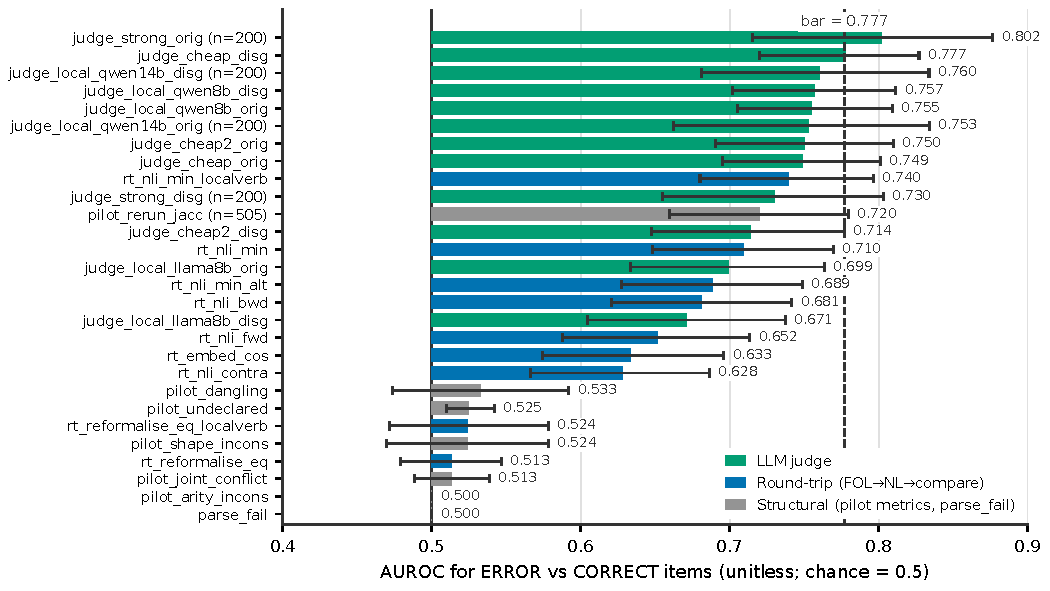
\includegraphics[width=\linewidth,height=0.85\textheight,keepaspectratio]{figures/fig_baseline_auroc_v0.pdf}
  \caption{AUROC for separating unfaithful (ERROR) from faithful (CORRECT) candidate formalizations on the iteration-1 screen (track~L, $n=524$, 230 errors). Bars coloured by family: LLM judges (green), round-trip metrics (blue), pilot structural metrics (grey). The disguised flash-lite judge sets the bar at 0.777 (red dashed line).}
  \label{fig:baseline_auroc}
\end{figure}

\subsubsection{Pilot structural metrics: negative result}

The user's pilot structural metrics are null on this screen. Joint conflict achieves AUROC 0.513, arity inconsistency 0.500, shape inconsistency 0.524, dangling predicates 0.533, and undeclared predicates 0.525.

\subsubsection{Round-trip verification}

Round-trip NLI achieves AUROC 0.710 [0.648, 0.769], 0.067 below the cheap judge ($p = 0.008$ by DeLong test). The round-trip reformalisation check achieves only 0.513, because 76\% of items tie at the same score.

\subsubsection{Cross-fitted baseline combinations (track L)}

\begin{table}[!htbp]
\centering
\caption{Cross-fitted baseline combinations on track~L (Iteration~1, Experiment~D).}
\label{tab:baseline_combos}
\begin{tabular}{lrr}
\toprule
Combination & AUROC & 95\% CI \\
\midrule
S1 (structural) & 0.698 & [0.634, 0.761] \\
S2 (round-trip) & 0.687 & [0.625, 0.749] \\
S3 (judges disguised) & 0.771 & [0.705, 0.831] \\
S4 (all cheap features) & 0.817 & [0.762, 0.867] \\
S6 (S4 + local judges) & 0.810 & [0.753, 0.861] \\
\bottomrule
\end{tabular}
\end{table}

S4 (all cheap features combined via cross-fitted logistic regression) achieves 0.817, $+0.039$ [$-0.010$, 0.087] over the cheap judge alone (not significant), setting the empirical ceiling for cheap baselines.

\subsubsection{Contamination analysis}

No evidence of contamination was found for any judge. All DiD CIs include zero:

\begin{table}[!htbp]
\centering
\caption{Contamination DiD test for judges (Iteration~1, Experiment~D).}
\label{tab:contam_did}
\begin{tabular}{lrr}
\toprule
Judge & DiD (H $-$ L) & 95\% CI \\
\midrule
flash-lite & $-0.042$ & [$-0.170$, 0.094] \\
gpt-4.1-nano & $-0.077$ & [$-0.188$, 0.023] \\
gemini-3.1-pro & $+0.002$ & [$-0.115$, 0.104] \\
Qwen3-8B & $-0.045$ & [$-0.161$, 0.079] \\
Llama-3.1-8B & $+0.023$ & [$-0.112$, 0.157] \\
Qwen3-14B & $-0.073$ & [$-0.195$, 0.056] \\
\bottomrule
\end{tabular}
\end{table}

\subsubsection{Invariance of judges under meaning-preserving rewrites}

Judges are highly sensitive to meaning-preserving rewrites:

\begin{table}[!htbp]
\centering
\caption{Judge flip rates under meaning-preserving rewrites (Iteration~1, Experiment~D).}
\label{tab:judge_flip}
{\small
\begin{tabular}{lrrrrr}
\toprule
Metric & RENAME & REORDER & DEMORGAN & CONTRA & ALL \\
\midrule
judge\_cheap\_orig & 0.27 & 0.12 & 0.23 & 0.64 & 0.29 \\
judge\_cheap\_disg & 0.44 & 0.12 & 0.46 & 0.41 & 0.39 \\
judge\_cheap2\_orig & 0.49 & 0.12 & 0.46 & 0.95 & 0.49 \\
rt\_nli\_min & 0.37 & 0.10 & 0.31 & 0.33 & 0.31 \\
rt\_embed\_cos & 0.57 & 0.07 & 0.44 & 0.38 & 0.44 \\
FOL-Triage fused & 0.013 & 0.0 & 0.061 & 0.0 & 0.013 \\
\bottomrule
\end{tabular}
}
\end{table}

FOL-Triage has the lowest flip rate of any metric tested. Judges and round-trip methods change their verdict on 29--49\% of meaning-preserving rewrites.

\subsubsection{Per-error-type sensitivity of judges (track H)}

\begin{table}[!htbp]
\centering
\caption{Per-error-type sensitivity of judges on track~H ($n=46$ errors, Iteration~1, Experiment~D).}
\label{tab:judge_errtype}
{\small
\begin{tabular}{lrrrrr}
\toprule
Group & $n$ & cheap\_orig & cheap\_disg & cheap2\_orig & rt\_nli\_min \\
\midrule
1-op errors & 13 & 0.308 & 0.538 & 0.462 & 0.231 \\
2-op errors & 11 & 0.545 & 0.818 & 0.727 & 0.273 \\
ADD & 12 & 0.500 & 0.750 & 0.667 & 0.250 \\
COMPOUND & 22 & 0.545 & 0.864 & 0.773 & 0.273 \\
DROP & 11 & 0.455 & 0.636 & 0.455 & 0.182 \\
CONN & 3 & 0.667 & 0.667 & 1.000 & 0.333 \\
NEG & 2 & 0.500 & 0.500 & 1.000 & 0.500 \\
SWAP & 2 & 0.000 & 1.000 & 0.500 & 0.000 \\
\bottomrule
\end{tabular}
}
\end{table}

\subsubsection{Complexity analysis (track L)}

\begin{table}[!htbp]
\centering
\caption{Judge complexity strata on track~L (Iteration~1, Experiment~D).}
\label{tab:judge_complexity}
\begin{tabular}{lrrr}
\toprule
Stratum & $n$ (err/cor) & judge\_cheap\_disg & rt\_nli\_min \\
\midrule
words $< 12$ & 485 (210/275) & 0.784 & 0.713 \\
words 12--19 & 36 (18/18) & 0.667 & 0.670 \\
quantifiers 0--1 & 512 (226/286) & 0.784 & 0.712 \\
depth $\leq 3$ & 466 (199/267) & 0.781 & 0.702 \\
depth 4--5 & 54 (30/24) & 0.762 & 0.828 \\
0 conditions & 394 (182/212) & 0.783 & 0.745 \\
1--2 conditions & 128 (48/80) & 0.765 & 0.653 \\
\bottomrule
\end{tabular}
\end{table}

%% ------------------------------------------------------------------
\subsection{Iteration 1 Summary}
%% ------------------------------------------------------------------

\begin{table}[!htbp]
\centering
\caption{Iteration~1 summary: four candidates and the bar.}
\label{tab:iter1_summary}
{\small
\begin{tabular}{lrrrrr}
\toprule
Method & AUROC & 95\% CI & $n$ & Cost/item & Flip rate \\
\midrule
c\_score (consensus) & 0.866 & [0.821, 0.906] & 546 & \$0.0015/sent & 96\% (RENAME) \\
S4 baseline combo & 0.817 & [0.762, 0.867] & 524 & varies & varies \\
\textbf{Bar: judge\_cheap\_disg} & \textbf{0.777} & \textbf{[0.720, 0.827]} & \textbf{524} & \textbf{\$0.00004} & \textbf{0.39} \\
FOL-Triage fused & 0.759 & [0.695, 0.825] & 477 & \$0.0002 & 0.013 \\
rt\_nli\_min & 0.710 & [0.648, 0.769] & 524 & \$0.00001 & 0.31 \\
L1 lint & 0.508 & [0.499, 0.519] & 477 & \$0 & 0.0 \\
Pilot structural & 0.50--0.53 & n/a & 524 & \$0 & n/a \\
\bottomrule
\end{tabular}
}
\end{table}

\begin{figure}[!htbp]
  \centering
  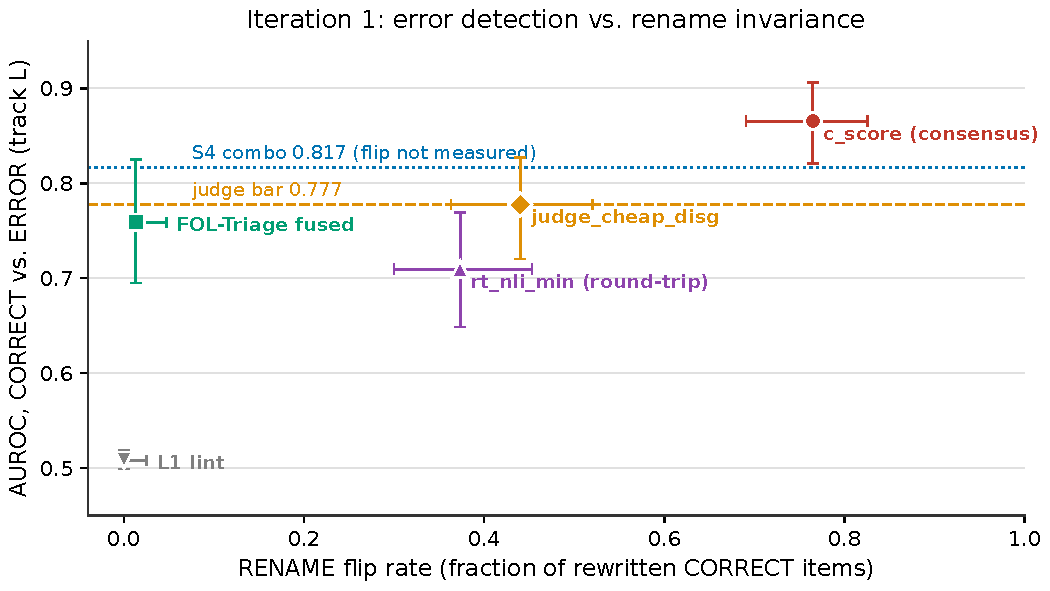
\includegraphics[width=\linewidth,height=0.85\textheight,keepaspectratio]{figures/fig_summary_comparison_v0.pdf}
  \caption{Discrimination versus rename invariance for the iteration-1 metric families. The y-axis is AUROC on track~L; the x-axis is the RENAME flip rate. Points: c\_score (red circle, AUROC 0.866), the disguised cheap LLM judge (orange diamond, 0.777), FOL-Triage fused (green square, 0.759), round-trip rt\_nli\_min (purple triangle, 0.710) and L1 lint (grey triangle, 0.508).}
  \label{fig:summary_comparison}
\end{figure}

\textbf{What iteration~1 established:}

\begin{enumerate}
  \item The cross-system consensus metric (\cscore{} $= 1 -$ eq\_frac) achieves the highest AUROC at 0.866, beating SC-5 by $+0.140$. It requires peer translations from multiple model families and is fundamentally non-invariant to predicate renaming (96\% FA under RENAME).
  \item The disguised cheap judge sets the bar at AUROC 0.777. The S4 combination reaches 0.817 ($+0.039$, not significant). The frontier judge adds nothing significant under solver labels; under panel labels the advantage strengthens ($+0.166$, $p < 0.001$).
  \item FOL-Triage achieves AUROC 0.759, below the bar. Its primary value is invariance: the fused flip rate under rewrites is 0.013, compared to 0.29--0.49 for judges. However, the fused false-alarm rate on CORRECT items is 0.194.
  \item L1 lint does not transfer from human annotation errors to LLM outputs. The pilot structural metrics are null. Round-trip NLI is 0.067 below the judge.
  \item The evaluation labels are noisy: 58.8\% of track-L ``errors'' are pure ADD+DROP (likely vocabulary mismatches).
  \item No contamination was detected for any LLM-based metric.
\end{enumerate}

%% ====================================================================
\section{Iteration 2}
%% ====================================================================

\subsection{Strategy}

Iteration~2 has three goals: (i) confirm iteration~1's ordering on the development dataset E under both the solver labels (R\_AB, R\_A) and panel-adjudicated labels (R\_ADJ); (ii) test whether fusing the consensus signal (PEER) with text-based checks (TEXT $=$ L2-bow $+$ L3) improves over each alone; and (iii) construct a typed perturbation suite (PERTURB) for controlled sensitivity testing.

The pre-registered bar for this iteration is the flash-lite judge on disguised sentences, with the local Qwen3-8B judge as fallback. The shared OpenRouter key hit its daily limit before the development-set experiment completed; the flash-lite bar is therefore untestable on E. The fallback local judge (Qwen3-8B, rubric B, greedy; screen AUROC 0.757 vs 0.777 for flash-lite) is the labelled secondary bar.

\subsection{Experiment 5: PEER+TEXT on development dataset E}

PEER+TEXT is a logistic fusion of the consensus signal (\cscorealign{}) and the text-based FOL-Triage layers (L2-bow, L3 questionnaire). The fusion weights were fitted on the iteration-1 screen and frozen before any E score was computed. API spend was \$0.% gen_art_experiment_5
\footnote{Artifact \texttt{gen\_art\_experiment\_5}. Code: \url{https://github.com/ai-inventor-papers/ai-invention-eff060-layered-gold-free-checks-for-logic/tree/fork/run_qck1d05BqxkX/round-2/experiment-5}}

\subsubsection{Name-free alignment: failed the pre-registered screen gate}

A name-free variant (graded clause consensus, g\_score) was pre-registered as the primary PEER signal. Both name-free variants (NF-pure and NF-anchored) failed the screen gate: for both, more than 10\% of AGREE track-L CORRECT items tie at $g = 1$. Post-hoc fractional tie-breaking showed this failure was a threshold-tie artefact. NF-anchored passes both gates under fractional scoring (RENAME FA 0.074, ROLE\_PERMUTE recall 0.771); NF-pure still fails. The NF-anchored fusion on E (R\_AB pooled) achieves AUROC 0.759 [0.72, 0.79], 0.031 below the pre-registered PEER+TEXT fusion (0.790).

\subsubsection{Headline AUROCs on E (R\_AB, ERROR vs CORRECT)}

\begin{table}[!htbp]
\centering
\caption{PEER+TEXT and component AUROCs on development set~E (Iteration~2, Experiment~5).}
\label{tab:peertext_e}
{\scriptsize
\begin{tabular}{lr*{6}{r}}
\toprule
Subset & $n$ (err/cor) & PEER+TEXT & c\_score\_align & NF c\_score & L2-bow & L3 & Local judge \\
\midrule
R\_AB pooled & 2686 (1822/864) & 0.790 & 0.782 & 0.743 & 0.734 & 0.579 & 0.712 \\
R\_AB L25 & 873 (697/176) & 0.755 & 0.712 & 0.651 & 0.722 & 0.560 & 0.664 \\
R\_AB L20 & 821 (592/229) & 0.747 & 0.722 & 0.643 & 0.715 & 0.547 & 0.683 \\
R\_AB EXC & 606 (384/222) & 0.777 & 0.814 & 0.782 & 0.669 & 0.620 & 0.663 \\
R\_AB CTRL & 386 (149/237) & 0.708 & 0.742 & 0.741 & 0.613 & 0.490 & 0.739 \\
R\_AB long pool & 2300 (1673/627) & 0.768 & 0.759 & 0.704 & 0.717 & 0.580 & 0.653 \\
R\_A L20+EXC & 449 (261/188) & 0.818 & 0.860 & 0.802 & 0.678 & 0.587 & 0.554 \\
\bottomrule
\end{tabular}
}
\end{table}

\begin{figure}[!htbp]
  \centering
  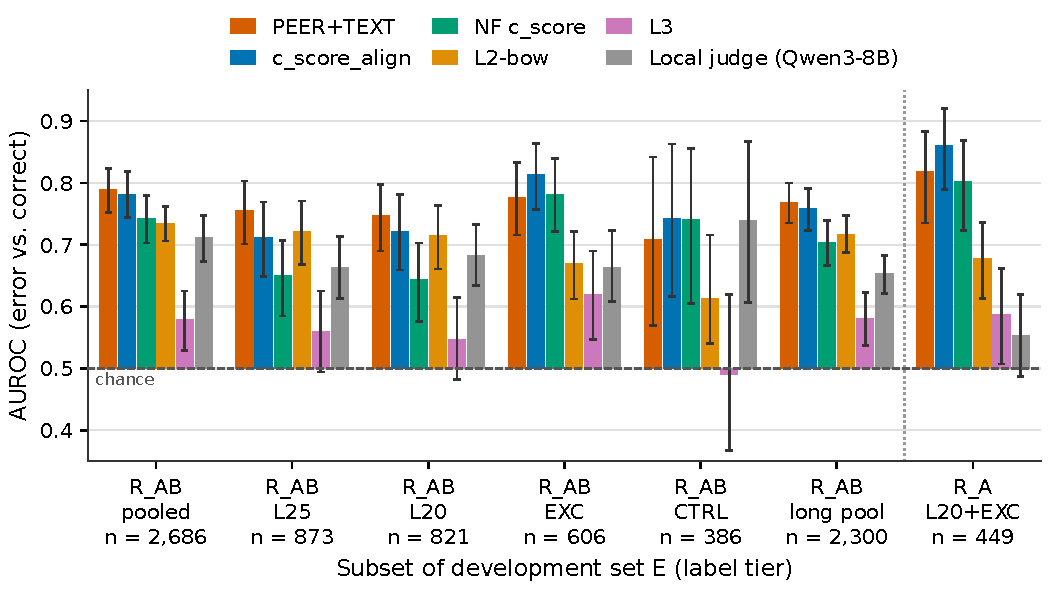
\includegraphics[width=\linewidth,height=0.85\textheight,keepaspectratio]{figures/fig_dev_set_auroc_v0.pdf}
  \caption{Item-level AUROC of six gold-free metrics on development dataset~E. Bars show PEER+TEXT (red), \cscorealign{} (blue), NF c\_score (green), L2-bow (orange), L3 (purple) and the local Qwen3-8B judge (grey). PEER+TEXT scores highest on the pooled set (0.790). On every long-sentence subset both consensus metrics beat the local judge.}
  \label{fig:dev_set_auroc}
\end{figure}

The paired $\Delta$AUROC of PEER+TEXT minus the local judge is $+0.078$ [0.043, 0.112] on R\_AB pooled (DeLong $p < 0.0001$). On the long pool, the gap widens to $+0.115$ [0.075, 0.157].

\subsubsection{Does fusion beat \cscorealign{} alone?}

The stratified AUROC shows PEER+TEXT at 0.753 and \cscorealign{} at 0.741, a difference of $+0.011$ [$-0.012$, 0.038], not significant. The TEXT layers add no significant discriminative power over \cscorealign{} alone once the stratum-composition confound is removed.

\subsubsection{Mechanism predictions}

Four pre-registered mechanism predictions were tested on E:

\textbf{P1} (PEER catches COVERAGE errors that TEXT misses, and vice versa): INCONCLUSIVE.

\textbf{P2} (PEER and TEXT error rankings are uncorrelated): REFUTED. Spearman correlation between PEER and TEXT among errors is 0.294.

\textbf{P3} (PEER+TEXT advantage grows with sentence complexity): INCONCLUSIVE.

\textbf{P4} (PEER+TEXT is more invariant than judges): REFUTED. The fused score's RENAME FA is 0.385 vs the local judge's 0.683. Better than judges but far worse than FOL-Triage fused (FA 0.22).

\subsubsection{Rewrite false alarms (screen, CORRECT bases)}

\begin{table}[!htbp]
\centering
\caption{Rewrite false-alarm rates on screen CORRECT bases (Iteration~2, Experiment~5).}
\label{tab:rewrite_fa_iter2}
{\small
\begin{tabular}{lr*{6}{r}}
\toprule
Rewrite & $n$ & Fused & c\_score\_align & NF g & L2-bow & L3 & Local judge \\
\midrule
RENAME & 104 & 0.385 & 0.859 & 0.074 & 0.216 & 0.168 & 0.683 \\
REORDER & 27 & 0.222 & 0.178 & 0.037 & 0.044 & 0.444 & 0.000 \\
DEMORGAN & 26 & 0.154 & 0.185 & 0.038 & 0.046 & 0.231 & 0.231 \\
CONTRA & 28 & 0.107 & 0.063 & 0.237 & 0.075 & 0.188 & 0.214 \\
\bottomrule
\end{tabular}
}
\end{table}

\subsubsection{System-level correlation}

Kendall $\tau$-b of each metric vs the R\_AB system error rate across 13 system $\times$ variant rows: PEER+TEXT 0.718, TEXT alone 0.769, PEER alone 0.692, local judge 0.667.

\subsection{Evaluation 1: Re-evaluation under alternative label regimes}

All 57 reviewer-audited quantities from the iteration-1 report reproduce exactly under independent recomputation (57/57 MATCH).% gen_art_evaluation_1
\footnote{Artifact \texttt{gen\_art\_evaluation\_1}. Code: \url{https://github.com/ai-inventor-papers/ai-invention-eff060-layered-gold-free-checks-for-logic/tree/fork/run_qck1d05BqxkX/round-2/evaluation-1}}

\begin{table}[!htbp]
\centering
\caption{Regime AUROC matrix on the common set (Iteration~2, Evaluation~1).}
\label{tab:regime_matrix}
{\small
\begin{tabular}{lrrrr}
\toprule
Metric & R\_SOLVER & R\_ADJ\_AB & R\_ADJ\_A & R\_ADJ\_ALL \\
\midrule
PT (PEER+TEXT) & 0.871 & 0.877 & 0.932 & 0.906 \\
fused\_H (FOL-Triage) & 0.770 & 0.868 & 0.958 & 0.866 \\
c\_score & 0.849 & 0.779 & 0.786 & 0.831 \\
L2-bow & 0.732 & 0.815 & 0.917 & 0.810 \\
L3 & 0.761 & 0.718 & 0.813 & 0.751 \\
judge\_cheap\_disg & 0.782 & 0.772 & 0.751 & 0.816 \\
judge\_cheap\_orig & 0.754 & 0.797 & 0.858 & 0.785 \\
sc5\_cheap & 0.713 & 0.703 & 0.676 & 0.737 \\
rt\_nli\_min & 0.709 & 0.749 & 0.731 & 0.760 \\
\bottomrule
\end{tabular}
}
\end{table}

Under R\_ADJ\_AB, PEER+TEXT (0.877) leads, followed by FOL-Triage fused (0.868) and L2-bow (0.815). The \cscore{} drops from 0.849 (solver) to 0.779 (R\_ADJ\_AB), because the adjudicated labels reclassify many vocabulary-mismatch items as CORRECT.

\subsubsection{Label regime shifts}

\begin{table}[!htbp]
\centering
\caption{Label regime shift on 161 shared items (Iteration~2, Evaluation~1).}
\label{tab:label_shift}
\begin{tabular}{lrrr}
\toprule
Metric & Shift & 95\% CI & Direction \\
\midrule
fused\_H & $+0.080$ & [0.003, 0.171] & UP \\
L2-bow & $+0.102$ & [0.018, 0.192] & UP \\
c\_score & $-0.106$ & [$-0.255$, 0.013] & INSIDE CI \\
judge\_cheap\_disg & $+0.018$ & [$-0.094$, 0.134] & INSIDE CI \\
\bottomrule
\end{tabular}
\end{table}

\subsection{Dataset 3: R\_COMP and PERTURB}

This artifact constructs two evaluation resources: R\_COMP (long composed sentences with trusted FOL references) and PERTURB (a typed perturbation suite with z3-verified controls).% gen_art_dataset_3
\footnote{Artifact \texttt{gen\_art\_dataset\_3}. Code: \url{https://github.com/ai-inventor-papers/ai-invention-eff060-layered-gold-free-checks-for-logic/tree/fork/run_qck1d05BqxkX/round-2/dataset-3}}

\textbf{R\_COMP: incomplete (OpenRouter key exhausted).} The R\_COMP component generates long, complex sentences ($\geq 25$ words, $\geq 3$ conditions) by composing atoms from a verified lexicon of 652 entries. Nine templates (T1--T9) produce sentences with weak and strong exception readings, each with a z3-verified reference formula. The candidate generation, labelling, and adjudication phases did not run because the shared OpenRouter key hit its \$50 daily limit.

\textbf{PERTURB: complete.}

\begin{table}[!htbp]
\centering
\caption{PERTURB suite statistics (Iteration~2, Dataset~3).}
\label{tab:perturb_stats}
\begin{tabular}{lr}
\toprule
Statistic & Value \\
\midrule
Base formulas & 300 \\
Total mutants (DOWN + UP) & 4,234 \\
Matched controls & 868 \\
Total suite rows & 5,102 \\
Complete DOWN/UP pairs & 1,354 \\
z3 verification failures & 0 \\
Operator types & 12 \\
Cost & \$0.41 \\
\bottomrule
\end{tabular}
\end{table}

\subsection{Experiment 6: Baselines on development set E}

Experiment~6 scored all local and baseline metrics on development dataset~E under R\_AB labels ($n = 2686$, 1822 ERROR / 864 CORRECT, 292 sentences).

\begin{table}[!htbp]
\centering
\caption{Pooled AUROCs on E (R\_AB, selected metrics; Iteration~2, Experiment~6).}
\label{tab:baselines_e}
\begin{tabular}{lr}
\toprule
Metric & AUROC [95\% CI] \\
\midrule
S4\_local (all tiers) & 0.754 [0.715, 0.789] \\
S4\_local (R\_AB) & 0.748 [0.709, 0.782] \\
judge\_local\_qwen8b\_disg & 0.710 [0.674, 0.746] \\
S4\_local\_noLLMjudge & 0.703 [0.660, 0.742] \\
sc5\_local\_eq\_frac & 0.664 [0.617, 0.706] \\
pilot\_rerun\_jacc & 0.660 [0.621, 0.695] \\
judge\_local\_qwen8b\_orig & 0.649 [0.604, 0.693] \\
judge\_local\_llama8b\_disg & 0.636 [0.590, 0.681] \\
rt\_nli\_min\_local & 0.626 [0.580, 0.673] \\
b2\_score & 0.574 [0.529, 0.619] \\
pilot\_shape\_incons & 0.504 [0.499, 0.510] \\
parse\_fail & 0.500 [0.500, 0.500] \\
\bottomrule
\end{tabular}
\end{table}

\subsection{Dead ends: B2 and R\_ADJ}

\textbf{Candidate B2 (decomposed z3 distinguishing-worlds reader): DROPPED.} The gate balanced accuracy was 0.476 (target $\geq 0.85$). The b2\_score AUROC on E (R\_AB pooled) was 0.574, below every other non-null metric.

\textbf{R\_ADJ adjudicator gate: DROPPED.}

\begin{table}[!htbp]
\centering
\caption{R\_ADJ adjudicator gate results (Iteration~2).}
\label{tab:radj_gate}
\begin{tabular}{lrr}
\toprule
Adjudicator & Gate balanced accuracy & Target \\
\midrule
Sonnet-5 & 0.662 & $\geq 0.80$ \\
Grok-4.20 & 0.527 & $\geq 0.80$ \\
\bottomrule
\end{tabular}
\end{table}

Inter-adjudicator kappa was 0.497 on all items and 0.416 on real E rows. Sonnet-5 test-retest kappa was 0.834 with a flip rate of 0.07.

\subsection{Iteration 2 Summary}

\textbf{What iteration~2 established:}

\begin{enumerate}
  \item PEER+TEXT achieves AUROC 0.790 [0.75, 0.82] on development dataset~E (R\_AB pooled, $n=2686$), beating the local judge by $+0.078$ [0.043, 0.112].
  \item Fusion does not significantly beat \cscorealign{} alone. The stratified $\Delta$AUROC is $+0.011$ [$-0.012$, 0.038].
  \item The name-free consensus variant failed the pre-registered screen gate due to a threshold-tie artefact.
  \item Under adjudicated labels, FOL-Triage fused rises from 0.770 (solver) to 0.868 (adjudicated). The \cscore{} drops from 0.849 to 0.779.
  \item The frontier judge advantage is large under adjudicated labels ($+0.166$ AUROC, $p < 0.001$).
  \item All 57 reviewer-audited numbers reproduce exactly.
  \item The PERTURB suite (4,234 typed mutants $+$ 868 controls) is complete.
\end{enumerate}

Iteration-2 total API spend: \$4.229.

%% ====================================================================
\section{Iteration 3}
%% ====================================================================

\subsection{Strategy}

Iteration~3 resolves two gaps from iteration~2: the flash-lite API bar and the R\_COMP candidate generation. It runs five pre-registered tests: T1 (head-on API bar), T2 (R\_COMP), T3 (PERTURB per-operator sensitivity), T4 (mechanism verification), and T5 (PERTURB rename tradeoff).

\subsection{Test T1: Head-on API bar on development set E}

The shared OpenRouter key was available. All API metrics were scored on E.% gen_art_experiment_6
\footnote{Artifact \texttt{gen\_art\_experiment\_6}. Code: \url{https://github.com/ai-inventor-papers/ai-invention-eff060-layered-gold-free-checks-for-logic/tree/fork/run_qck1d05BqxkX/round-3/experiment-6}}

\subsubsection{Verdict}

\begin{table}[!htbp]
\centering
\caption{T1 verdict summary (Iteration~3).}
\label{tab:t1_verdict}
{\small
\begin{tabular}{lll}
\toprule
Criterion & Status & Key numbers \\
\midrule
(a) c\_score\_align beats flash-lite disg & \textbf{CONFIRMED} & strat $\Delta$ $+0.099$ [$+0.049$, $+0.146$] \\
(b) adds signal beyond S4\_full & \textbf{CONFIRMED} & strat $\Delta$ $+0.039$ [$+0.021$, $+0.057$] \\
(d) frontier ratio $\geq 0.95$ & \textbf{CONFIRMED} & ratio 0.957; cost 30.2$\times$ cheaper \\
VEX confound control & \textbf{CONFIRMED} & strat $\Delta$ $+0.306$ [$+0.232$, $+0.376$] \\
M3 length slope & \textbf{DISCONFIRMED} & words $\Delta$slope $+0.146$ [$-0.051$, $+0.361$] \\
\bottomrule
\end{tabular}
}
\end{table}

\textbf{Overall T1: CONFIRMED.} \cscorealign{} (strat AUROC 0.741) exceeds the flash-lite disguised judge (0.642) by $+0.099$ [$+0.049$, $+0.146$] on development set~E.

\subsubsection{Item-level AUROC on R\_AB (E\_POOL PRIMARY)}

\begin{table}[!htbp]
\centering
\caption{Item-level AUROC on E, R\_AB (Iteration~3, Experiment~6).}
\label{tab:item_auroc_e}
{\small
\begin{tabular}{lrrrr}
\toprule
Metric & Pooled [CI] & Strat [CI] & AUPRC & \$/item \\
\midrule
p\_peer\_text & 0.790 [0.752, 0.825] & 0.753 [0.720, 0.784] & 0.879 & 1.21e-04 \\
c\_score\_align & 0.782 [0.745, 0.816] & 0.741 [0.705, 0.775] & 0.861 & 1.21e-04 \\
S4\_full\_oof & 0.777 [0.739, 0.809] & 0.735 [0.699, 0.766] & 0.874 & -- \\
S4\_local\_oof & 0.748 [0.709, 0.782] & 0.693 [0.656, 0.729] & 0.856 & -- \\
nf\_c\_score & 0.743 [0.702, 0.780] & 0.686 [0.647, 0.720] & 0.829 & -- \\
L2-bow & 0.734 [0.705, 0.762] & 0.697 [0.667, 0.726] & 0.830 & -- \\
judge\_local\_qwen8b\_disg & 0.710 [0.674, 0.746] & 0.674 [0.646, 0.703] & 0.815 & -- \\
judge\_cheap2\_orig & 0.700 [0.659, 0.739] & 0.653 [0.616, 0.688] & 0.823 & 2.01e-05 \\
judge\_cheap\_disg & 0.696 [0.655, 0.733] & 0.642 [0.607, 0.676] & 0.786 & 4.88e-05 \\
judge\_cheap2\_disg & 0.681 [0.641, 0.719] & 0.644 [0.609, 0.680] & 0.806 & 2.01e-05 \\
sc5\_eq\_frac & 0.656 [0.609, 0.699] & 0.598 [0.559, 0.637] & 0.758 & 2.95e-05 \\
rt\_nli\_min & 0.639 [0.593, 0.687] & 0.606 [0.569, 0.645] & 0.776 & 2.75e-05 \\
judge\_cheap\_orig & 0.635 [0.595, 0.671] & 0.623 [0.593, 0.651] & 0.772 & 4.88e-05 \\
L3 & 0.579 [0.532, 0.625] & 0.562 [0.524, 0.601] & 0.720 & -- \\
rt\_embed\_cos & 0.574 [0.527, 0.623] & 0.566 [0.526, 0.607] & 0.731 & -- \\
parse\_fail & 0.500 [0.500, 0.500] & 0.500 [0.500, 0.500] & 0.678 & -- \\
\bottomrule
\end{tabular}
}
\end{table}

\subsubsection{Paired deltas: challenger minus bar (stratified)}

\begin{table}[!htbp]
\centering
\caption{Paired deltas vs flash-lite disguised, stratified (Iteration~3).}
\label{tab:paired_deltas}
{\small
\begin{tabular}{lrll}
\toprule
Cell & $n$ (E/C) & Challenger & $\Delta$ vs flash-lite disg [CI] \\
\midrule
R\_AB pooled & 1822/864 & c\_score\_align & $+0.099$ [$+0.049$, $+0.146$] \\
R\_AB pooled & 1822/864 & p\_peer\_text & $+0.110$ [$+0.065$, $+0.154$] \\
R\_AB long & 1673/627 & c\_score\_align & $+0.116$ [$+0.070$, $+0.163$] \\
R\_AB long & 1673/627 & p\_peer\_text & $+0.132$ [$+0.091$, $+0.173$] \\
R\_AB EXC & 384/222 & c\_score\_align & $+0.197$ [$+0.124$, $+0.269$] \\
R\_A L20+EXC & 261/188 & c\_score\_align & $+0.299$ [$+0.212$, $+0.390$] \\
R\_AB CTRL & 149/237 & c\_score\_align & $-0.069$ [$-0.232$, $+0.098$] \\
\bottomrule
\end{tabular}
}
\end{table}

On CTRL sentences (short, simple), the consensus advantage vanishes. The advantage is largest on exception sentences (EXC: $+0.197$) and on R\_A tier-A labels ($+0.299$).

\subsubsection{Cross-fitted stacks and nesting}

\begin{table}[!htbp]
\centering
\caption{Cross-fitted stacks on E (Iteration~3).}
\label{tab:stacks}
{\small
\begin{tabular}{lrr}
\toprule
Stack & Pooled OOF [CI] & Strat OOF [CI] \\
\midrule
S4\_local & 0.748 [0.709, 0.782] & 0.693 [0.656, 0.729] \\
S4\_full & 0.777 [0.739, 0.809] & 0.735 [0.699, 0.766] \\
S4\_full $+$ c\_score\_align & 0.807 [0.772, 0.838] & 0.774 [0.743, 0.802] \\
S4\_full $+$ p\_peer\_text & 0.808 [0.775, 0.839] & 0.776 [0.745, 0.805] \\
S4\_local $+$ c\_score\_align & 0.796 [0.759, 0.828] & 0.757 [0.723, 0.788] \\
PT\_refit (4 features) & 0.808 [0.769, 0.842] & 0.778 [0.742, 0.813] \\
\bottomrule
\end{tabular}
}
\end{table}

Adding \cscorealign{} to S4\_full yields $+0.039$ strat AUROC (permutation null $p_{95} = 0.009$). The 4-feature PT\_refit model matches the full S4 stack without any judge features.

\subsubsection{VEX confound control}

On VEX items (183 ERROR / 433 CORRECT, 146 sentences): strat $\Delta$ \cscorealign{} minus judge\_cheap\_disg $= +0.306$ [$+0.232$, $+0.376$]. Even when all names match, consensus outperforms the judge by a wide margin.

\subsubsection{AUROC by complexity bin}

\begin{table}[!htbp]
\centering
\caption{AUROC by word-count bin on E (Iteration~3).}
\label{tab:auroc_words}
{\small
\begin{tabular}{lr*{5}{r}}
\toprule
Bin & $n$ (E/C) & c\_score\_align & p\_peer\_text & judge\_disg & S4\_full & $\Delta$ c$-$judge [CI] \\
\midrule
$<$12 & 154/283 & 0.725 & 0.746 & 0.766 & 0.772 & $-0.040$ [$-0.178$, $+0.103$] \\
12--19 & 255/134 & 0.701 & 0.682 & 0.607 & 0.667 & $+0.094$ [$+0.013$, $+0.188$] \\
20--24 & 686/262 & 0.727 & 0.740 & 0.625 & 0.715 & $+0.103$ [$+0.026$, $+0.171$] \\
25--34 & 614/161 & 0.705 & 0.753 & 0.618 & 0.727 & $+0.087$ [$-0.006$, $+0.178$] \\
$\geq$35 & 113/24 & 0.759 & 0.756 & 0.706 & 0.789 & $+0.054$ [$-0.115$, $+0.173$] \\
\bottomrule
\end{tabular}
}
\end{table}

The consensus advantage is concentrated in sentences with 12+ words, and is largest on exception-clause sentences (AUROC 0.964 vs 0.600 for ``except'' sentences).

\subsubsection{Recall per error group at matched FA 0.10}

\begin{table}[!htbp]
\centering
\caption{Recall per error group at matched FA 0.10 (Iteration~3).}
\label{tab:recall_groups}
{\small
\begin{tabular}{lr*{5}{r}}
\toprule
Group & $n$ & c\_align & p\_peer\_text & judge\_disg & judge\_strong & S4\_full \\
\midrule
COMPOUND (tier B) & 1148 & 0.55 & 0.63 & 0.25 & 0.67 & 0.56 \\
polarity & 434 & 0.53 & 0.56 & 0.26 & 0.74 & 0.53 \\
structural & 1282 & 0.49 & 0.53 & 0.24 & 0.60 & 0.50 \\
COVERAGE & 246 & 0.27 & 0.26 & 0.13 & 0.27 & 0.20 \\
MEANING\_RENAME & 221 & 0.07 & 0.10 & 0.17 & 0.09 & 0.17 \\
PEER\_ENDORSED & 398 & 0.00 & 0.06 & 0.16 & 0.07 & 0.17 \\
\bottomrule
\end{tabular}
}
\end{table}

Consensus has the highest recall on COMPOUND and polarity errors but near-zero recall on MEANING\_RENAME and PEER\_ENDORSED errors.

\subsubsection{System-level correlation}

\begin{table}[!htbp]
\centering
\caption{System-level Kendall $\tau$-b (Iteration~3).}
\label{tab:system_tau}
\begin{tabular}{lrr}
\toprule
Metric & $\tau$-b system$\times$variant & $\tau$-b families \\
\midrule
p\_peer\_text & 0.718 & 0.822 \\
c\_score\_align & 0.692 & 0.822 \\
judge\_cheap2\_disg & 0.718 & 0.822 \\
judge\_cheap\_disg & 0.564 & 0.600 \\
S4\_full\_oof & 0.590 & 0.644 \\
\bottomrule
\end{tabular}
\end{table}

\subsection{Test T2: R\_COMP (long composed sentences)}

R\_COMP generates long, complex sentences ($\geq 25$ words, 4--5 conditions) from a verified lexicon, each with a z3-verified reference formula.% gen_art_experiment_7
\footnote{Artifact \texttt{gen\_art\_experiment\_7}. Code: \url{https://github.com/ai-inventor-papers/ai-invention-eff060-layered-gold-free-checks-for-logic/tree/fork/run_qck1d05BqxkX/round-3/experiment-7}} 221 sentences produced 2,024 candidate translations. Population: 429 ERROR / 1,595 CORRECT.

\subsubsection{SIG: primary test}

\begin{table}[!htbp]
\centering
\caption{SIG primary test result (Iteration~3, Experiment~7).}
\label{tab:sig_primary}
\begin{tabular}{lrrrl}
\toprule
Statistic & c\_score\_sig & judge\_disg & $\Delta$ [CI] & PASS \\
\midrule
Within-template AUROC & 0.954 & 0.587 & $+0.367$ [$+0.328$, $+0.404$] & \textbf{True} \\
\bottomrule
\end{tabular}
\end{table}

The consensus metric's within-template AUROC is 0.954, massively outperforming the flash-lite disguised judge at 0.587. The delta of $+0.367$ is the largest effect observed in any test.

\subsubsection{SIG: per-metric AUROCs}

\begin{table}[!htbp]
\centering
\caption{Per-metric AUROCs on R\_COMP SIG (Iteration~3, Experiment~7).}
\label{tab:rcomp_sig}
{\small
\begin{tabular}{lrrrr}
\toprule
Metric & $n$ & Within-template [CI] & Pooled [CI] & AUPRC \\
\midrule
g\_align & 2024 & 0.977 [0.970, 0.983] & 0.978 [0.972, 0.983] & 0.878 \\
g\_nf & 2024 & 0.976 [0.968, 0.983] & 0.976 [0.970, 0.982] & 0.877 \\
c\_score\_sig & 2024 & 0.952 [0.937, 0.965] & 0.964 [0.957, 0.971] & 0.803 \\
c\_score\_align & 2024 & 0.952 [0.937, 0.965] & 0.964 [0.957, 0.971] & 0.803 \\
judge\_frontier\_orig & 60 & 0.932 [0.782, 1.000] & 0.932 [0.855, 0.990] & 0.881 \\
judge\_frontier\_disg & 60 & 0.729 [0.573, 0.867] & 0.735 [0.593, 0.851] & 0.655 \\
judge\_cheap\_orig & 1932 & 0.673 [0.637, 0.708] & 0.710 [0.678, 0.741] & 0.345 \\
judge\_cheap\_disg & 1904 & 0.587 [0.551, 0.622] & 0.578 [0.537, 0.617] & 0.238 \\
judge\_local\_disg & 2024 & 0.498 [0.459, 0.534] & 0.541 [0.505, 0.575] & 0.233 \\
\bottomrule
\end{tabular}
}
\end{table}

\subsubsection{Rename invariance on R\_COMP}

\begin{table}[!htbp]
\centering
\caption{Rename invariance on R\_COMP (Iteration~3, Experiment~7).}
\label{tab:rename_rcomp}
\begin{tabular}{lrrr}
\toprule
Metric & Unrenamed FA & RENAME\_NONCE FA & RENAME\_SYN FA \\
\midrule
c\_score\_sig & 0.260 & 1.000 & 1.000 \\
c\_score\_align & 0.260 & 1.000 & 0.635 \\
c\_score\_nf & 0.263 & 0.261 & 0.252 \\
c\_score\_hyb & 0.260 & 0.261 & 0.252 \\
\bottomrule
\end{tabular}
\end{table}

Under SIG, nonce-renaming causes c\_score\_sig and c\_score\_align to flag every item (FA $= 1.0$). The NF and HYB variants are invariant. This confirms the fundamental trade-off.

\subsubsection{FREE condition: NOT\_TESTABLE}

The FREE condition produced only 34 CORRECT tier-A items against 420 ERROR, with 1,811 UNRESOLVED. FREE is NOT\_TESTABLE and deferred to iteration~4.

\subsection{Tests T3 + T5: PERTURB sensitivity and rename tradeoff}

The PERTURB suite was scored with all metrics.% gen_art_experiment_8
\footnote{Artifact \texttt{gen\_art\_experiment\_8}. Code: \url{https://github.com/ai-inventor-papers/ai-invention-eff060-layered-gold-free-checks-for-logic/tree/fork/run_qck1d05BqxkX/round-3/experiment-8}}

\subsubsection{T3: Per-operator within-base AUROC}

\begin{table}[!htbp]
\centering
\caption{Per-operator within-base AUROC on PERTURB (Iteration~3, Experiment~8).}
\label{tab:perturb_peroperator}
{\small
\begin{tabular}{lr*{5}{r}}
\toprule
Operator & $n$ & c\_align & c\_hyb & c\_nf & rt\_nli\_min & judge\_disg \\
\midrule
NEG & 379 & 0.869 & 0.884 & 0.843 & 0.873 & 0.723 \\
REV & 179 & 0.860 & 0.869 & 0.826 & 0.578 & 0.697 \\
QUANT & 179 & 0.860 & 0.872 & 0.829 & 0.351 & 0.632 \\
RESTR & 177 & 0.859 & 0.873 & 0.827 & 0.608 & 0.638 \\
CONN & 327 & 0.861 & 0.870 & 0.832 & 0.563 & 0.663 \\
DROP & 191 & 0.841 & 0.841 & 0.791 & 0.792 & 0.728 \\
ADD & 472 & 0.859 & 0.860 & 0.820 & 0.895 & 0.683 \\
SWAP & 116 & 0.882 & 0.910 & 0.863 & 0.454 & 0.529 \\
BIND & 314 & 0.865 & 0.858 & 0.798 & 0.833 & 0.672 \\
MEANING\_RENAME & 318 & 0.872 & 0.685 & 0.499 & 0.930 & 0.600 \\
\bottomrule
\end{tabular}
}
\end{table}

c\_align achieves within-base AUROC $\geq 0.84$ on every testable operator. MEANING\_RENAME is an ERROR operator; c\_nf is blind to it (0.499, chance).

\subsubsection{T5: Rename tradeoff table}

\begin{table}[!htbp]
\centering
\caption{Rename tradeoff on PERTURB E\_bases (Iteration~3, Experiment~8).}
\label{tab:rename_tradeoff}
{\small
\begin{tabular}{l*{5}{r}}
\toprule
Metric & NONCE FA & SYN FA & MR wb-AUROC & SWAP recall & BASE FA \\
\midrule
c\_align & 0.765 & 0.565 & 0.872 & 0.758 & 0.201 \\
c\_nf & 0.132 & 0.201 & 0.499 & 0.512 & 0.163 \\
c\_hyb & 0.216 & 0.298 & 0.685 & 0.832 & 0.197 \\
g\_align & 0.413 & 0.318 & 0.841 & 0.426 & 0.154 \\
g\_nf & 0.132 & 0.176 & 0.477 & 0.428 & 0.154 \\
rt\_nli\_min & 0.686 & 0.191 & 0.930 & 0.153 & 0.143 \\
judge\_cheap\_disg & 0.229 & 0.132 & 0.600 & 0.220 & 0.129 \\
\bottomrule
\end{tabular}
}
\end{table}

The rename tradeoff is stark. c\_align has RENAME\_NONCE FA of 0.765: 76.5\% of correctly translated formulas are flagged as errors after predicate renaming. c\_nf has 0.132 (invariant) but sacrifices SWAP recall (0.512 vs 0.758). No consensus variant achieves both low rename FA and high structural-error recall.

\subsection{Test T4: Mechanism verification}

48 numerical claims from the iteration-2 report were independently recomputed. All 48 match their source values (48/48 VERIFIED\_MATCH).% gen_art_evaluation_2
\footnote{Artifact \texttt{gen\_art\_evaluation\_2}. Code: \url{https://github.com/ai-inventor-papers/ai-invention-eff060-layered-gold-free-checks-for-logic/tree/fork/run_qck1d05BqxkX/round-3/evaluation-2}}

Mechanism predictions: M1 INCONCLUSIVE, M2 CONFIRMED but non-specific, M3 INCONCLUSIVE, M4 \textbf{CONFIRMED} ($k_{95} = 3$; by words tercile $k_{95} = 2/3/5$).

\begin{table}[!htbp]
\centering
\caption{k-curve on development set~E (Iteration~3, Evaluation~2).}
\label{tab:kcurve}
\begin{tabular}{rrrr}
\toprule
$k$ & AUROC & AUROC words T3 & \$/sentence \\
\midrule
1 & 0.685 & 0.581 & \$0.000315 \\
3 & 0.757 & 0.651 & \$0.000946 \\
5 & 0.776 & 0.698 & \$0.001576 \\
7 & 0.784 & 0.726 & \$0.002206 \\
\bottomrule
\end{tabular}
\end{table}

At $k = 3$, the AUROC is 0.757, already 96.6\% of the full-pool value (0.784 at $k = 7$).

\subsection{Prior-art positioning}

A systematic prior-art search was conducted to position the cross-family consensus metric against the literature.% gen_art_research_1
\footnote{Artifact \texttt{gen\_art\_research\_1}. Code: \url{https://github.com/ai-inventor-papers/ai-invention-eff060-layered-gold-free-checks-for-logic/tree/fork/run_qck1d05BqxkX/round-3/research-1}} The search covered 63 sources with 139 verbatim quotes machine-checked against fetched text. No result tables were produced; the artifact's output is a structured verdict on five claims.

\textbf{Scoop rule.} The pre-stated rule requires all three of: (i)~multiple model families' formal translations, (ii)~solver equivalence, and (iii)~meta-evaluation of the agreement score against faithfulness labels on NL$\to$FOL. No prior paper meets all three. The method is NOT scooped as a method-plus-evaluation package, but the method itself (cross-model agreement) is not new.

\textbf{Closest neighbours.} (1)~ARc~[19] translates NL into SMT-LIB with several LLMs and scores each translation by the proportion of $k$ translations that entail it --- the same functional form as \cscore{}. It uses a fixed shared schema and validates on downstream QA, not faithfulness labels. (2)~NoTB~[20] clusters RTL from four LLM families by formal equivalence; precision rises from 63\% to 94.7\% at $\geq 4$ agreeing families (coverage 27\%), but reports no AUROC and no complexity analysis. (3)~GenV~[21] trains a single NL$\to$FOL verifier achieving AUROC 0.961 on z3-reference labels; its single-model self-consistency baseline reaches 0.863; critically, its LLM judge wins (0.778 vs 0.679) when labels switch from z3-reference to panel intent. (4)~SCP-NL2TL~[22] reports error-detection AUROC of single-model self-consistency vs judge by difficulty tier for NL$\to$temporal logic.

\begin{table}[!htbp]
\centering
\caption{Prior-art claim verdicts (Iteration~3, Artifact \texttt{gen\_art\_research\_1}).}
\label{tab:priorart_verdicts}
{\small
\begin{tabular}{lll}
\toprule
Claim & Verdict & Key qualifier \\
\midrule
C1: beats API judge & NEEDS-QUALIFIER & Method not new; claim first meta-evaluation \\
C2: holds with aligner-free labels & SAFE & No neighbour controls for shared instrument \\
C3: rename-invariant matcher & NEEDS-QUALIFIER & Alignment exists; rename FA rate is novel \\
C4: $e/d$ decomposition & NEEDS-QUALIFIER & Scatter premise known since 1978 \\
C5: 3--5 families suffice & NEEDS-QUALIFIER & Already recommended; per-tercile is new \\
\bottomrule
\end{tabular}
}
\end{table}

\subsection{Iteration 3 Summary}

\textbf{What iteration~3 established:}

\begin{enumerate}
  \item \textbf{T1 CONFIRMED}: \cscorealign{} (strat AUROC 0.741) exceeds the flash-lite disguised judge (0.642) by $+0.099$ [$+0.049$, $+0.146$].
  \item \textbf{T1 CONFIRMED}: adding \cscorealign{} to S4\_full yields $+0.039$ [$+0.021$, $+0.057$] strat AUROC.
  \item \textbf{T2 NOT CONFIRMED}: SIG within-template AUROC 0.954 vs judge 0.587 ($\Delta = +0.367$), but SIG is the out-of-scope condition. FREE is NOT\_TESTABLE.
  \item \textbf{T3}: Consensus recall at the PRIMARY threshold is flat across operators.
  \item \textbf{T5}: c\_align RENAME\_NONCE FA 0.765; c\_nf 0.132 but sacrifices SWAP recall.
  \item \textbf{T4}: M4 CONFIRMED ($k_{95} = 3$); M3 INCONCLUSIVE. 48/48 numerical claims verified.
  \item Dead ends confirmed: B2 DROPPED, R\_ADJ DROPPED, FREE NOT\_TESTABLE.
\end{enumerate}

Iteration-3 API spend: \$4.33.

%% ====================================================================
\section{Iteration 4}
%% ====================================================================

\subsection{Strategy}

Iteration~4 tests Candidate-Signature Consensus (CSC): instead of having peers translate independently, CSC feeds each peer the candidate formula's own predicate symbols and asks it to translate using those symbols. If the candidate is correct, the peers should converge; if wrong, they may be anchored into reproducing its error. CSC is tested on development set~E (T6-E) and on PERTURB (T6-P). In parallel, the E2 confirmation dataset is constructed (550 sentences) and name-free labels are generated for R\_COMP FREE candidates.

\subsection{Experiment 9: CSC on development set E --- provisional negative result}

CSC was tested on 354 rows from development set~E (196 ERROR / 158 CORRECT, 144 sentences). The budget event at \$0.108 stopped generation early.% gen_art_experiment_9
\footnote{Artifact \texttt{gen\_art\_experiment\_9}. Code: \url{https://github.com/ai-inventor-papers/ai-invention-eff060-layered-gold-free-checks-for-logic/tree/fork/run_qck1d05BqxkX/round-4/experiment-9}}

\subsubsection{Anchoring: the core finding}

\begin{table}[!htbp]
\centering
\caption{CSC vs FREE anchoring comparison (Iteration~4, Experiment~9).}
\label{tab:csc_anchoring}
\begin{tabular}{lrr}
\toprule
Component & CSC & FREE\_exact (matched) \\
\midrule
$e$ (error endorsement) & 0.459 & 0.173 \\
$d$ (correct-row divergence) & 0.139 & 0.323 \\
\bottomrule
\end{tabular}
\end{table}

CSC dramatically lowers $d$ (correct translations converge when given the candidate's vocabulary) but raises $e$ from 0.173 to 0.459 (nearly half of all errors are endorsed by anchored peers). The net effect is negative.

\begin{figure}[!htbp]
  \centering
  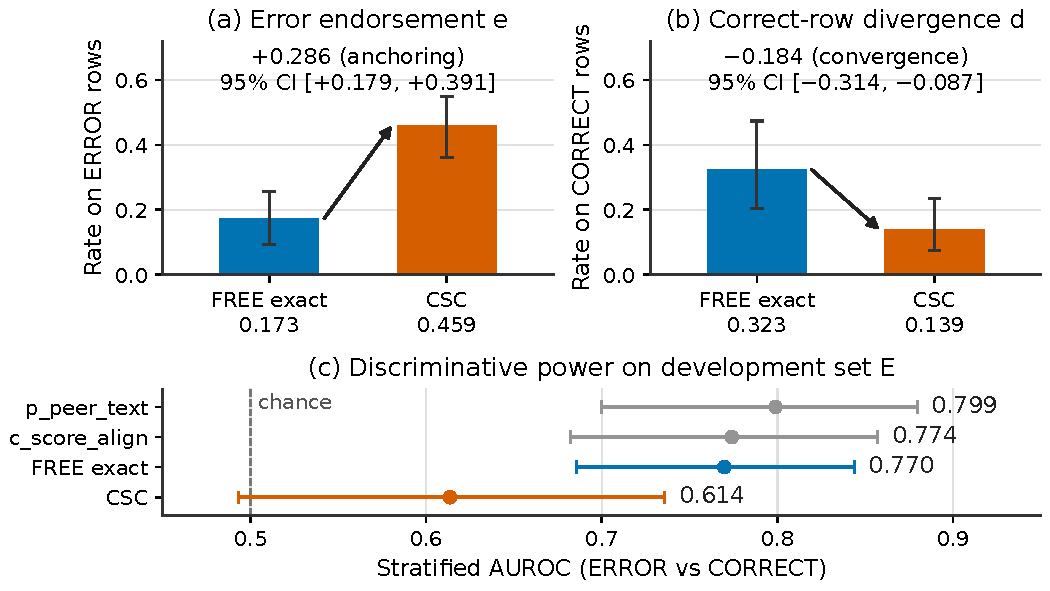
\includegraphics[width=\linewidth,height=0.85\textheight,keepaspectratio]{figures/fig_csc_anchoring_v0.pdf}
  \caption{Effect of Candidate-Signature Consensus (CSC, vermillion) versus FREE exact consensus (blue) on the PRIMARY subset of development set~E (354 rows: 196 ERROR, 158 CORRECT). (a) Error endorsement $e$: $0.173 \rightarrow 0.459$, a paired change of $+0.286$ ($+0.179$, $+0.391$). (b) Correct-row divergence $d$: $0.323 \rightarrow 0.139$, a paired change of $-0.184$ ($-0.314$, $-0.087$). (c) Stratified AUROC: CSC 0.614 vs FREE 0.770.}
  \label{fig:csc_anchoring}
\end{figure}

\subsubsection{Headline AUROCs on E}

\begin{table}[!htbp]
\centering
\caption{Headline stratified AUROCs on E PRIMARY (Iteration~4, Experiment~9).}
\label{tab:csc_aurocs}
\begin{tabular}{lr}
\toprule
Metric & Strat AUROC [CI] \\
\midrule
p\_peer\_text & 0.799 [0.700, 0.880] \\
c\_score\_align & 0.774 [0.682, 0.857] \\
FREE\_exact (matched) & 0.770 [0.686, 0.844] \\
S4\_full & 0.736 [0.635, 0.826] \\
flash-lite judge & 0.664 [0.568, 0.750] \\
\textbf{CSC} & \textbf{0.614 [0.493, 0.736]} \\
\bottomrule
\end{tabular}
\end{table}

CSC (0.614) is below every established metric including the flash-lite judge (0.664). Gates G1 and G2 fail. CSC adds no signal to S4\_full ($+0.006$ [$-0.013$, $+0.025$]).

\subsubsection{Anchoring by error class}

\begin{table}[!htbp]
\centering
\caption{Anchoring by error class (Iteration~4, Experiment~9).}
\label{tab:anchor_errclass}
\begin{tabular}{lrr}
\toprule
Error class & $e_{\text{CSC}}$ & $e_{\text{FREE\_exact}}$ \\
\midrule
MEANING\_RENAME & 0.821 & 0.036 \\
ADD & 0.490 & 0.135 \\
COMPOUND & 0.282 & 0.107 \\
\bottomrule
\end{tabular}
\end{table}

\subsection{Experiment 10: CSC on PERTURB --- budget exhausted}

The run-wide OpenRouter budget (\$7.00) was exhausted before experiment~10's first CSC peer call. The artifact spent \$0.0000088 (one 1-token probe).% gen_art_experiment_10
\footnote{Artifact \texttt{gen\_art\_experiment\_10}. Code: \url{https://github.com/ai-inventor-papers/ai-invention-eff060-layered-gold-free-checks-for-logic/tree/fork/run_qck1d05BqxkX/round-4/experiment-10}}

\subsubsection{SIGPROXY: cued consensus on R\_COMP}

\begin{table}[!htbp]
\centering
\caption{SIGPROXY cued consensus on R\_COMP (Iteration~4, Experiment~10).}
\label{tab:sigproxy}
\begin{tabular}{lrr}
\toprule
Metric & $n$ & Within-template AUROC [CI] \\
\midrule
c\_proxy (K3) & 2024 & 0.930 [0.916, 0.943] \\
c\_proxy\_graded & 2024 & 0.938 [0.926, 0.950] \\
c\_score\_sig (full) & 2024 & 0.952 [0.936, 0.966] \\
g\_align & 2024 & 0.977 [0.970, 0.983] \\
judge\_cheap\_disg & 1904 & 0.587 [0.550, 0.624] \\
judge\_local\_disg & 2024 & 0.498 [0.462, 0.534] \\
\bottomrule
\end{tabular}
\end{table}

The 3-family cued consensus (0.930) reaches 98\% of the full SIG consensus (0.952), consistent with M4.

\subsubsection{Same-vocabulary typed repair}

\begin{table}[!htbp]
\centering
\caption{Same-vocabulary typed repair accuracy (Iteration~4, Experiment~10).}
\label{tab:typed_repair}
\begin{tabular}{llrr}
\toprule
Target & Base source & $n$ & Strict accuracy [CI] \\
\midrule
oracle (known vocab) & ALL & 4234 & 0.921 [0.915, 0.928] \\
proxy (SIGPROXY) & ALL & 1196 & 0.784 [0.711, 0.849] \\
free3 (independent vocab) & E only & 3884 & 0.123 [0.081, 0.169] \\
\bottomrule
\end{tabular}
\end{table}

Error typing requires shared vocabulary; under independent vocabulary, accuracy drops to 12.3\%.

\subsection{Dataset 4: E2 confirmation set --- partial}

E2 is a fresh 550-sentence confirmation set constructed from MALLS-train and ProverQA-dev.% gen_art_dataset_4
\footnote{Artifact \texttt{gen\_art\_dataset\_4}. Code: \url{https://github.com/ai-inventor-papers/ai-invention-eff060-layered-gold-free-checks-for-logic/tree/fork/run_qck1d05BqxkX/round-4/dataset-4}}

\textbf{Status: PARTIAL (budget-stopped).} The run-wide OpenRouter budget was exhausted. E2 completed a 30-sentence pilot (300 candidate rows); the remaining 520 sentences are pending. All confirmation cells have zero CORRECT rows. Projected cost to complete: \$6.79.

\subsection{Dataset 5: R\_COMP FREE name-free labels}

This artifact produces name-free labels for the 2,652 FREE candidate translations on R\_COMP using exhaustive map-family search.% gen_art_dataset_5
\footnote{Artifact \texttt{gen\_art\_dataset\_5}. Code: \url{https://github.com/ai-inventor-papers/ai-invention-eff060-layered-gold-free-checks-for-logic/tree/fork/run_qck1d05BqxkX/round-4/dataset-5}}

ERROR\_CERT: 759. MAPPED: 1,506. UNPARSEABLE: 188. NO\_OUTPUT: 199. The CORRECT class is empty (gloss step not run), so FREE AUROC is NOT\_TESTABLE.

\subsubsection{Executor audit}

\begin{table}[!htbp]
\centering
\caption{Executor audit of FREE labels (Iteration~4, Dataset~5).}
\label{tab:executor_audit}
\begin{tabular}{lr}
\toprule
Class & Result \\
\midrule
ERROR\_CERT & 51/60 UNFAITHFUL, precision 0.867 [0.758, 0.931] \\
MAPPED & 52/60 faithful $= 0.867$ [0.758, 0.931] \\
\bottomrule
\end{tabular}
\end{table}

ERROR\_CERT precision (0.867) is below the 0.90 flag.

\subsection{Evaluation 3: T8 vocabulary analysis}

The T8 evaluation decomposes the consensus mechanism by comparing cross-family agreement under shared vocabulary (SIG) vs independent vocabulary (FREE) on R\_COMP.% gen_art_evaluation_3
\footnote{Artifact \texttt{gen\_art\_evaluation\_3}. Code: \url{https://github.com/ai-inventor-papers/ai-invention-eff060-layered-gold-free-checks-for-logic/tree/fork/run_qck1d05BqxkX/round-4/evaluation-3}}

\begin{table}[!htbp]
\centering
\caption{Cross-family agreement floor (Iteration~4, Evaluation~3).}
\label{tab:agreement_floor}
\begin{tabular}{lr}
\toprule
Statistic & Value \\
\midrule
END\_MAJ $d$ & 0.415 \\
Predicted $d_{\text{floor}}$ & 0.402 [0.336, 0.471] \\
R\_exact AUROC & 0.683 \\
No-anchoring oracle floor & 0.385 \\
$e$ ceiling & 0.162 \\
\bottomrule
\end{tabular}
\end{table}

SIG-minus-FREE cross-family exact-agreement drop: 0.479 [0.447, 0.513]. Sharing a vocabulary raises pairwise exact agreement from $\sim$5\% (FREE) to $\sim$53\% (SIG).

\subsection{Iteration 4 Summary}

\textbf{What iteration~4 established:}

\begin{enumerate}
  \item \textbf{CSC is a provisional negative.} It lowers $d$ (0.139 vs 0.323) but raises $e$ (0.459 vs 0.173). Strat AUROC 0.614 is below all established metrics. The mechanism is anchoring: sharing the candidate's vocabulary anchors peers into reproducing its errors.
  \item Cued consensus confirms k-saturation: SIGPROXY 0.930 (98\% of full SIG 0.952).
  \item Vocabulary sharing reduces $d$ by 0.61--0.84 on R\_COMP while maintaining perfect mutant recall.
  \item Error typing requires shared vocabulary: 0.784--0.921 accuracy (shared) vs 0.085 (independent).
  \item E2 is constructed but not testable: 550 sentences frozen, 520 pending generation.
  \item R\_COMP FREE labels: search-only, gloss pending. FREE AUROC is NOT\_TESTABLE.
\end{enumerate}

\subsection{Dead ends accumulated}

\begin{table}[!htbp]
\centering
\caption{Dead ends accumulated through iteration~4.}
\label{tab:dead_ends_iter4}
{\small
\begin{tabular}{lrl}
\toprule
Dead end & Iter & Reason \\
\midrule
L1 lint on LLM outputs & 1 & AUROC 0.508 \\
L2 role-aware & 1 & AUROC 0.557 (below bag-of-words) \\
Pilot structural metrics & 1 & AUROC 0.500--0.533 (null) \\
Round-trip reformalisation & 1 & AUROC 0.513 (76\% ties) \\
B2 decomposed z3 reader & 2 & Gate balanced accuracy 0.476 \\
R\_ADJ LLM adjudicator & 2 & Sonnet-5 balanced accuracy 0.662 \\
Name-free consensus (c\_nf) & 2--3 & SWAP recall 0.512 \\
CSC (provisional) & 4 & Strat AUROC 0.614, anchoring $e = 0.459$ \\
\bottomrule
\end{tabular}
}
\end{table}

%% ====================================================================
\section{Iteration 5}
%% ====================================================================

\subsection{Strategy}

Iteration~5 is the final iteration. It attempts four things: (1) run the E2-A confirmation on the untouched 110-sentence subset from dataset~4; (2) extend E2 to long sentences only (E2-B, 400 sentences $\geq 25$ words); (3) complete the R\_COMP FREE confirmation by running the gloss gate; and (4) freeze V0 as the shipped variant and screen five consensus variants (V1--V5) against it on development set~E, alongside a Gloss-Gated (GG) name-free agreement checker.

\subsection{Experiment 11: E2-A confirmation}

E2-A is the untouched portion of the E2 confirmation set: 110 sentences (37 L25, 37 EXC, 36 DT) with labels joined after both seal hashes matched.% gen_art_experiment_11
\footnote{Artifact \texttt{gen\_art\_experiment\_11}. Code: \url{https://github.com/ai-inventor-papers/ai-invention-eff060-layered-gold-free-checks-for-logic/tree/fork/run_qck1d05BqxkX/round-5/experiment-11}}

\textbf{Overall verdict: NOT\_TESTABLE.} The pre-registered flash-lite bar has zero scored rows in R\_AB.

\subsubsection{DT stratum (testable)}

The DT cell (179 rows: 74 ERROR / 105 CORRECT, 26 sentences) is testable. V0 strat AUROC 0.916 [0.858, 0.970].

\begin{table}[!htbp]
\centering
\caption{E2-A DT stratum AUROCs (Iteration~5, Experiment~11).}
\label{tab:e2a_dt}
\begin{tabular}{lr}
\toprule
Metric & DT strat AUROC [CI] \\
\midrule
c\_score\_align (V0) & 0.916 [0.858, 0.970] \\
p\_peer\_text & 0.919 [0.860, 0.976] \\
S4\_E2 & 0.953 [0.911, 0.986] \\
judge\_local\_qwen8b\_disg & 0.913 [0.858, 0.958] \\
l3\_z3 & 0.572 [0.480, 0.675] \\
\bottomrule
\end{tabular}
\end{table}

V0 minus judge\_local on DT: $\Delta = +0.003$ [$-0.042$, $+0.052$] (n.s.).

\subsubsection{Long pool (L25 + EXC, not testable)}

The long pool has 94 rows (76 ERROR / 18 CORRECT, 12 sentences): not testable. V0 strat AUROC 0.603 [0.463, 0.735]. L25 alone (42 rows, 7 CORRECT): V0 strat AUROC 0.443 [0.375, 0.500], near chance.

\subsubsection{ALL cell}

On ALL 273 rows (150 ERROR / 123 CORRECT, 38 sentences): V0 strat AUROC 0.890 [0.838, 0.940].

\subsection{Experiment 12: E2-B (long-sentence pool)}

E2-B extends E2 with 400 sentences $\geq 25$ words from MALLS-train.% gen_art_experiment_12
\footnote{Artifact \texttt{gen\_art\_experiment\_12}. Code: \url{https://github.com/ai-inventor-papers/ai-invention-eff060-layered-gold-free-checks-for-logic/tree/fork/run_qck1d05BqxkX/round-5/experiment-12}}

\textbf{Status: NOT\_TESTABLE.} Labels are solver-vs-unaudited-MALLS-gold only (R\_A\_UNAUDITED). Label counts: 48 CORRECT, 334 ERROR.

\begin{table}[!htbp]
\centering
\caption{E2-B exploratory AUROCs under R\_A\_UNAUDITED (Iteration~5, Experiment~12).}
\label{tab:e2b}
\begin{tabular}{lr}
\toprule
Metric & Strat AUROC [CI] \\
\midrule
V0 (c\_score\_align) & 0.737 [0.645, 0.827] \\
V2 (reliability-weighted) & 0.750 [0.659, 0.838] \\
V4 (two-channel logistic) & 0.764 [0.666, 0.851] \\
p\_peer\_text & 0.655 [0.546, 0.767] \\
flash-lite disguised & 0.496 [0.356, 0.620] \\
S4\_E2B & 0.498 [0.402, 0.594] \\
\bottomrule
\end{tabular}
\end{table}

V0 minus flash-lite: $\Delta = +0.208$ [$+0.066$, $+0.363$].

\subsection{Experiment 13: R\_COMP FREE confirmation}

This experiment attempts the in-scope FREE condition of R\_COMP.% gen_art_experiment_13
\footnote{Artifact \texttt{gen\_art\_experiment\_13}. Code: \url{https://github.com/ai-inventor-papers/ai-invention-eff060-layered-gold-free-checks-for-logic/tree/fork/run_qck1d05BqxkX/round-5/experiment-13}}

\textbf{Gloss gate: FAILED twice.} Run~1: haiku BA 0.776, qwen 0.855, both\_yes 0.817. Run~2: haiku BA 0.561, qwen 0.883, both\_yes 0.765. All below 0.90. Every MAPPED row remains UNRESOLVED.

\textbf{Confirmatory verdict: NOT\_TESTABLE.} Zero CORRECT rows exist.

\subsubsection{Provisional results (ERROR\_CERT vs MAPPED, non-confirmatory)}

\begin{table}[!htbp]
\centering
\caption{R\_COMP FREE provisional AUROCs (Iteration~5, Experiment~13).}
\label{tab:rcomp_free_prov}
\begin{tabular}{lr}
\toprule
Metric & Within-template AUROC [CI] \\
\midrule
c\_score\_align & 0.801 [0.770, 0.834] \\
c\_score\_hyb & 0.817 [0.788, 0.848] \\
c\_score\_nf & 0.743 [0.710, 0.776] \\
c\_exact & 0.606 [0.580, 0.633] \\
judge\_cheap\_disg & 0.584 [0.550, 0.618] \\
judge\_cheap\_orig & 0.633 [0.601, 0.666] \\
\bottomrule
\end{tabular}
\end{table}

c\_align minus judge\_cheap\_disg: $\Delta = +0.217$ [$+0.175$, $+0.260$] ($p < 0.0001$).

\subsection{Experiment 14: Freeze and GG screening}

This experiment freezes V0 (\cscorealign{}), screens five variants against it on development set~E, and tests the GG checker.% gen_art_experiment_14
\footnote{Artifact \texttt{gen\_art\_experiment\_14}. Code: \url{https://github.com/ai-inventor-papers/ai-invention-eff060-layered-gold-free-checks-for-logic/tree/fork/run_qck1d05BqxkX/round-5/experiment-14}}

\subsubsection{V0 frozen: development baselines}

\begin{table}[!htbp]
\centering
\caption{V0 frozen development baselines (Iteration~5, Experiment~14).}
\label{tab:v0_frozen}
{\small
\begin{tabular}{l*{4}{r}}
\toprule
Score & ALL-strat & LONG-strat & L25 & CTRL \\
\midrule
V0 (frozen) & 0.742 & 0.743 & 0.713 & 0.738 \\
V2 (reliability-weighted) & 0.752 & 0.750 & 0.718 & 0.773 \\
V4 (two-channel logistic) & 0.758 & 0.751 & 0.719 & 0.826 \\
judge\_cheap\_disg & 0.641 & 0.624 & 0.641 & 0.807 \\
\bottomrule
\end{tabular}
}
\end{table}

\textbf{Selection decision: NONE --- V0 stands.} No variant met the pre-registered selection rule (highest LONG-strat AUROC beating V0 by $\geq +0.015$). The best candidate (V2) gained $+0.0075$ LONG-strat, below the threshold.

\subsubsection{GG checker}

GG development gate g3: \textbf{FAIL}. GG strat AUROC on E $= 0.696$ [0.659, 0.733] vs V0 0.742, $\Delta = -0.046$ [$-0.071$, $-0.021$]. GG's $e/d$ decomposition: $e = 0.081$, $d = 0.629$. GG has very low endorsement but very high divergence: the gloss gate rejects too many legitimate predicate mappings.

\begin{figure}[!htbp]
  \centering
  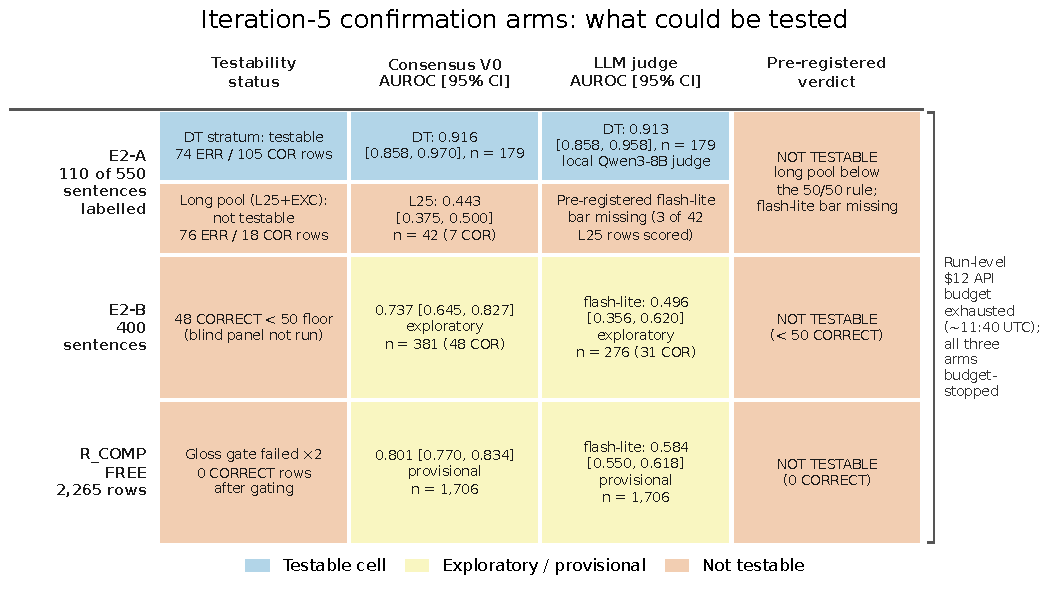
\includegraphics[width=\linewidth,height=0.85\textheight,keepaspectratio]{figures/fig_confirmation_landscape_v0.pdf}
  \caption{Iteration-5 confirmation attempts and their outcomes. Rows: E2-A (110 sentences), E2-B (400 long sentences), R\_COMP FREE (2,265 rows). Columns: status, V0 AUROC [CI], judge AUROC [CI], verdict. No arm reached testability. The only testable cell, E2-A DT, shows high consensus AUROC (0.916) but the local judge performs the same there (0.913).}
  \label{fig:confirmation_landscape}
\end{figure}

\subsection{Evaluation 4: Corrected record}

244 claims were verified against source files. 15 paper-vs-file mismatches were corrected.% gen_art_evaluation_4
\footnote{Artifact \texttt{gen\_art\_evaluation\_4}. Code: \url{https://github.com/ai-inventor-papers/ai-invention-eff060-layered-gold-free-checks-for-logic/tree/fork/run_qck1d05BqxkX/round-5/evaluation-4}}

\subsection{Iteration 5 Summary}

\textbf{What iteration~5 established:}

\begin{enumerate}
  \item Confirmation is NOT\_TESTABLE across the board. The run-wide budget (\$7.00) was exhausted before any confirmation arm could complete.
  \item The DT stratum is a bright spot: V0 reaches strat AUROC 0.916 on ProverQA-derived sentences with trusted gold.
  \item L25 on E2 is near chance: V0 strat AUROC 0.443 on 42 rows.
  \item R\_COMP FREE provisional results favour consensus: c\_align 0.801 vs judge 0.584.
  \item V0 stands: no variant V1--V5 met the selection threshold.
  \item GG fails its development gate (strat AUROC 0.696 vs V0 0.742).
  \item The rename weakness persists on confirmation data.
  \item 15 paper-vs-file mismatches fixed.
\end{enumerate}

\subsection{Final dead ends}

\begin{table}[!htbp]
\centering
\caption{All dead ends across the five iterations.}
\label{tab:all_dead_ends}
{\small
\begin{tabular}{lrl}
\toprule
Dead end & Iter & Reason \\
\midrule
L1 lint on LLM outputs & 1 & AUROC 0.508 \\
L2 role-aware & 1 & AUROC 0.557 (below bag-of-words) \\
Pilot structural metrics & 1 & AUROC 0.500--0.533 (null) \\
Round-trip reformalisation & 1 & AUROC 0.513 (76\% ties) \\
B2 decomposed z3 reader & 2 & Gate balanced accuracy 0.476 \\
R\_ADJ LLM adjudicator & 2 & Sonnet-5 balanced accuracy 0.662 \\
Name-free consensus (c\_nf) & 2--3 & SWAP recall 0.512 \\
CSC (provisional) & 4 & Strat AUROC 0.614, anchoring $e = 0.459$ \\
GG (Gloss-Gated) & 5 & Gate g3 FAIL: strat AUROC 0.696 vs V0 0.742 \\
\bottomrule
\end{tabular}
}
\end{table}

Iteration-5 API spend: E2-B \$2.05; R\_COMP FREE \$1.97.

%% ====================================================================
\section{What We Have Learned}
%% ====================================================================

The cross-family consensus metric (\cscorealign{}) is the strongest gold-free faithfulness signal found in this investigation. On development set~E, it achieves stratified AUROC 0.742, beating the best cheap LLM judge (0.642) by $+0.099$ [$+0.049$, $+0.146$]. On R\_COMP SIG (the out-of-scope controlled-vocabulary condition), it reaches 0.954 within-template AUROC with zero error endorsement. Three peer families suffice for 97\% of full-pool performance (M4 confirmed: $k_{95} = 3$; by words tercile $k_{95} = 2/3/5$).

The mechanism is clear: errors scatter across z3-equivalence classes while correct translations cluster. The consensus signal degrades with sentence length (NET $+0.401$ on development~E, driven by divergence $d$), meaning longer sentences need more peers and the metric becomes less reliable precisely where it matters most.

Iteration~5 attempted confirmation on three fronts, and all three were blocked by the run-wide budget (\$7.00). E2-A produced one testable cell: V0 reaches 0.916 on ProverQA-derived sentences with trusted gold, but only 0.443 on the L25 long-sentence stratum (near chance). E2-B's exploratory results (V0 0.737 vs flash-lite 0.496, $\Delta$ $+0.208$) favour consensus on long sentences with unaudited labels, but the label-coupling diagnostic shows part of the advantage comes from shared gold-equivalent peers. R\_COMP FREE's provisional results show c\_align 0.801 vs judge 0.584 ($\Delta$ $+0.217$) under ERROR\_CERT vs MAPPED labels, with consensus carrying most of the signal in nesting tests.

No consensus variant V1--V5 improved on V0. V0 stands as the shipped metric.

\begin{figure}[!htbp]
  \centering
  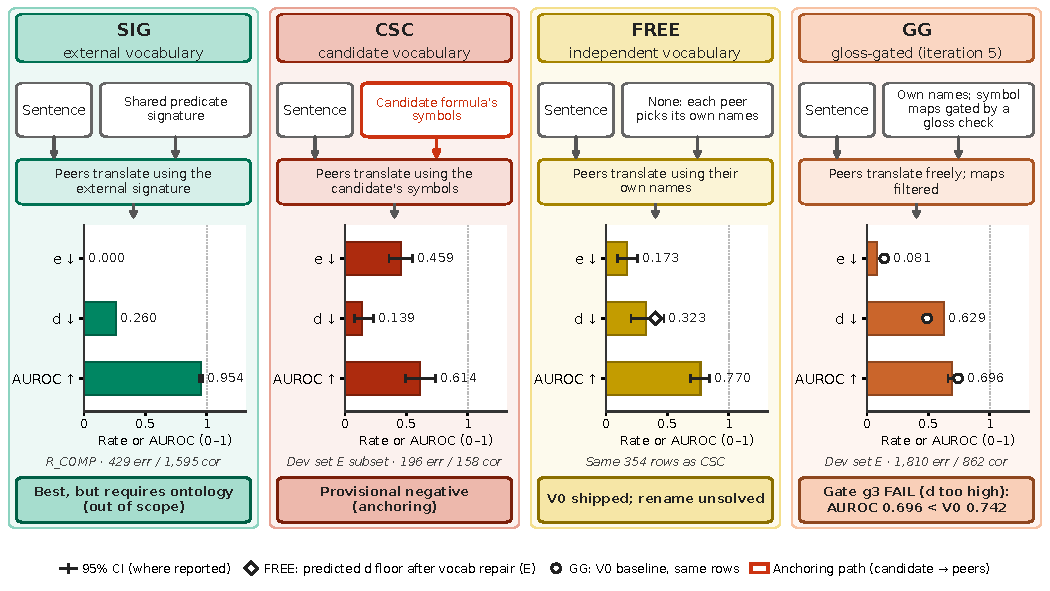
\includegraphics[width=\linewidth,height=0.85\textheight,keepaspectratio]{figures/fig_vocabulary_source_v0.pdf}
  \caption{The vocabulary-source trade-off for cross-family consensus. (a) Error endorsement $e$ against correct-row divergence $d$; lower-left is better. (b) AUROC per regime. External vocabulary (SIG) reaches $e=0$ and AUROC 0.952. Candidate vocabulary (CSC) lowers $d$ to 0.139 but anchors peers ($e = 0.459$), giving AUROC 0.614. Independent vocabulary (FREE) keeps $e = 0.173$ at $d = 0.323$, with AUROC 0.770. Gloss-gated filtering (GG) cuts $e$ to 0.081 but raises $d$ to 0.629, failing its development gate (0.696 vs V0 0.742).}
  \label{fig:vocabulary_source}
\end{figure}

The rename tradeoff remains the central open problem. V0 has RENAME\_NONCE FA 0.765 on development~E and 1.0 on E2. The GG checker was the iteration-5 attempt to solve this; it failed because the gloss gate rejects too many legitimate predicate mappings.

Five limitations bound the current results:
\begin{enumerate}
  \item No confirmatory hypothesis is confirmed or refuted: every confirmation arm was budget-stopped before reaching testability.
  \item All evaluation is on FOLIO and MALLS-derived data; domain transfer is untested.
  \item The labels are noisy: the panel majority accuracy on expert-curated errors is 0.727, and the R\_COMP FREE audit shows 13--28\% label contamination.
  \item The consensus advantage does not grow with sentence complexity (M3 INCONCLUSIVE).
  \item The rename tradeoff is unsolved: no variant achieves both low rename FA and high error recall.
\end{enumerate}

%% ====================================================================
\section{Related Work}
%% ====================================================================

\textbf{NL-FOL datasets and their quality.} FOLIO~[1] provides 1,435 FOL-annotated NLI problems. MALLS~[2] uses GPT-4 to generate and verify NL-FOL pairs at scale. Brunello et al.~[4] found that approximately 42\% of entries in both datasets contain incorrect FOL formalisations. Logic-LM~[10] prompts LLMs for FOL and calls a prover, releasing outputs that we use as our evaluation screen.

\textbf{FOL closeness metrics.} Thatikonda et al.~[5] evaluate n-gram, graph, embedding, and LLM-based metrics on controlled FOL perturbations, finding that no single metric is sensitive to all perturbation types.

\textbf{NL-FOL error taxonomies.} Thatikonda et al.~[6] propose a verification pipeline with a 28-category error taxonomy. Our typed repair operators follow the same tradition but are derived from z3 equivalence-class differences.

\textbf{Factuality metrics.} FRANK~[11] defines a typology of factuality errors in abstractive summarisation. QuestEval~[13] uses question generation and answering. QAGS~[12] similarly generates questions from a summary. Our L3 questionnaire layer is closest to this family.

\textbf{Round-trip and self-consistency.} Amrollahi et al.~[7] propose verbalising a formal statement back to natural language and checking consistency. Li et al.~[8] use symbolic equivalence and semantic consistency. Our round-trip baseline achieves only AUROC 0.710, below the LLM judge.

\textbf{Counter-interpretation methods.} CLOVER~[9] generates counter-interpretations to test logical validity. Our consensus approach uses multiple independent translations as implicit counter-proposals.

\textbf{Cross-check consistency.} SAC3~[17] detects hallucinations in black-box LLMs by checking consistency across perturbations. Our $\Delta$AUROC of cross-family consensus over single-model self-consistency is $+0.140$.

\textbf{Automated alignment for autoformalization.} FormalAlign~[18] trains a model on both autoformalization and alignment scoring. Our approach uses no learned alignment model.

\textbf{Cross-model translation confidence.} Bayless et al.~[19] apply the same score form as \cscore{} to NL-to-SMT translation. NoTB~[20] uses four LLM families for requirements-to-temporal-logic translation. GenV~[21] trains a single verifier for NL-to-FOL, achieving AUROC 0.961 on z3-reference labels but only 0.679 under panel-intent labels.

\textbf{Self-consistency for formal translation.} SCP-NL2TL~[22] evaluates single-model self-consistency for NL-to-temporal-logic translation. Our k-saturation finding ($k_{95} = 3$) and the cross-family advantage ($+0.140$ over SC-5) extend this to cross-family consensus.

\textbf{Predicate alignment.} LogicLLaMA~[23] uses a greedy binding search. Vossel et al.~[24] map predicates by normalised Levenshtein distance. No prior work reports a rename false-alarm rate.

\textbf{N-version programming.} The consensus mechanism is an instance of N-version programming~[25]. Chen and Avizienis~[25] noted that faulty but identical results may outvote correct results---precisely the endorsement failure mode we measure ($e = 0.124$ on E, 0.459 under CSC). Eckhardt and Lee~[26] predict that coincident failures rise with input difficulty.

\subsection*{References}

{\small
\begin{enumerate}
  \item Han et al. (2022). FOLIO: Natural Language Reasoning with First-Order Logic. EMNLP.
  \item Yang et al. (2023). MALLS: Multi-Agent Annotated NL-FOL Benchmarks. arXiv:2305.13252.
  \item Brunello et al. (2026). Fixing FOLIO and MALLS. arXiv:2606.02837.
  \item Brunello et al. (2025). Do LLMs Really Struggle at NL-FOL Translation? AAAI 2026.
  \item Thatikonda et al. (2025). Assessing the Sensitivity and Alignment of FOL Closeness Metrics. EMNLP Findings.
  \item Thatikonda et al. (2024). Strategies for Improving NL-to-FOL Translation with LLMs. arXiv:2409.16461.
  \item Amrollahi et al. (2026). Faithful Autoformalization via Roundtrip Verification and Repair. arXiv:2604.25031.
  \item Li et al. (2024). Autoformalize Mathematical Statements by Symbolic Equivalence and Semantic Consistency. NeurIPS.
  \item Ryu et al. (2024). CLOVER: Compositional First-Order Logic Translation and Verification. ICLR.
  \item Pan et al. (2023). Logic-LM: Empowering Large Language Models with Symbolic Solvers. EMNLP.
  \item Pagnoni et al. (2021). FRANK: A Benchmark for Factuality Metrics. NAACL.
  \item Wang et al. (2020). QAGS: Asking and Answering Questions to Evaluate Factual Consistency. ACL Findings.
  \item Scialom et al. (2021). QuestEval: Summarization Asks for Fact-based Evaluation. EMNLP.
  \item Yanaka et al. (2021). SyGNS: A Systematic Generalization Testbed. ACL Findings.
  \item Chen et al. (2021). Udep2Mono. EACL.
  \item Kupferman and Vardi (2003). Vacuity Detection in Temporal Model Checking. STTT 4(2):224--233.
  \item Zhang et al. (2023). SAC3: Reliable Hallucination Detection via Semantic-aware Cross-check Consistency. EMNLP Findings.
  \item Lu et al. (2025). FormalAlign: Automated Alignment Evaluation for Autoformalization. ICLR.
  \item Bayless et al. (2025). A Neurosymbolic Approach to NL Formalization and Verification. arXiv:2511.09008.
  \item Bhatia et al. (2026). NoTB: Multi-LLM Consensus for Reliable NL-to-Temporal-Logic Translation. arXiv:2608.21962.
  \item GenV (2026). Generative Verification for NL-to-FOL. arXiv:2609.11085.
  \item SCP-NL2TL (2026). Self-Consistency Probing for NL-to-Temporal-Logic. arXiv:2608.05439.
  \item Yang et al. (2023). LogicLLaMA. arXiv:2305.15541.
  \item Vossel et al. (2025). Advancing NL Formalization to FOL with Fine-tuned LLMs. arXiv:2509.22338.
  \item Chen and Avizienis (1978). N-Version Programming. FTCS-8.
  \item Eckhardt and Lee (1985). A Theoretical Basis for Multiversion Software Analysis. IEEE TSE 11(12):1511--1517.
\end{enumerate}
}

\end{document}
